\documentclass[11pt,a4paper]{article}

\usepackage[utf8]{inputenc}
\usepackage[T1]{fontenc}
\usepackage[french]{babel}
\usepackage{lmodern}
\usepackage{microtype}
\usepackage{geometry}
\usepackage{amsmath,amssymb,amsthm,mathtools}
\usepackage{xcolor}
\usepackage{graphicx}
\usepackage{hyperref}
\usepackage{enumitem}
\usepackage{booktabs}
\usepackage{listings}
\usepackage{tcolorbox}
\usepackage{tikz}
\usetikzlibrary{arrows.meta,positioning,fit,calc}
\usepackage{array}

\geometry{margin=2.4cm}
\hypersetup{
  colorlinks=true,
  linkcolor=blue!50!black,
  urlcolor=blue!50!black,
  citecolor=blue!50!black
}

\definecolor{codebg}{RGB}{248,248,248}
\definecolor{codeframe}{RGB}{215,215,215}
\definecolor{commentgreen}{RGB}{40,120,60}

\lstdefinestyle{pythoncourse}{
  language=Python,
  basicstyle=\ttfamily\small,
  keywordstyle=\color{blue!65!black}\bfseries,
  commentstyle=\color{commentgreen},
  stringstyle=\color{orange!55!black},
  showstringspaces=false,
  breaklines=true,
  frame=single,
  framerule=0.3pt,
  rulecolor=\color{codeframe},
  backgroundcolor=\color{codebg},
  columns=fullflexible,
  tabsize=2
}

\newtcolorbox{intuitionbox}{
  colback=blue!3,
  colframe=blue!45!black,
  title=Intuition,
  fonttitle=\bfseries,
  arc=2mm,
  boxrule=0.5pt
}

\newtcolorbox{definitionbox}[1]{
  colback=green!3,
  colframe=green!40!black,
  title=#1,
  fonttitle=\bfseries,
  arc=2mm,
  boxrule=0.5pt
}

\newtcolorbox{warningbox}{
  colback=orange!5,
  colframe=orange!65!black,
  title=Point d'attention,
  fonttitle=\bfseries,
  arc=2mm,
  boxrule=0.5pt
}

\theoremstyle{definition}
\newtheorem{definition}{Définition}[section]
\newtheorem{example}{Exemple}[section]
\theoremstyle{plain}
\newtheorem{theoreme}{Théorème}[section]
\newtheorem{proposition}{Proposition}[section]
\newtheorem{lemme}{Lemme}[section]
\newtheorem{corollaire}{Corollaire}[section]
\theoremstyle{remark}
\newtheorem{remark}{Remarque}[section]
\newtheorem{hypothese}{Hypothèse}[section]

% Convention francophone : on utilise "Démonstration" plutôt que "Proof"
\providecommand{\demonstrationname}{Démonstration}
\makeatletter
\renewenvironment{proof}[1][\demonstrationname]{\par
  \pushQED{\qed}%
  \normalfont \topsep6\p@\@plus6\p@\relax
  \trivlist
  \item[\hskip\labelsep
        \bfseries #1\@addpunct{.}]\ignorespaces
}{%
  \popQED\endtrivlist\@endpefalse
}
\makeatother

% Symbole d'indépendance probabiliste
\newcommand{\independent}{\perp\!\!\!\perp}

\newcommand{\R}{\mathbb{R}}
\newcommand{\N}{\mathbb{N}}
\newcommand{\E}{\mathbb{E}}
\newcommand{\Prob}{\mathbb{P}}
\newcommand{\Id}{\mathrm{Id}}
\newcommand{\dd}{\,\mathrm{d}}
\newcommand{\pp}{\text{p.p.}}
\newcommand{\ps}{\text{p.s.}}
\newcommand{\KLdiv}[2]{\KL\!\left(#1\,\middle\|\,#2\right)}
\newcommand{\loi}{\overset{\mathrm{loi}}{=}}
\DeclareMathOperator{\Var}{Var}
\DeclareMathOperator{\Cov}{Cov}
\DeclareMathOperator{\Law}{Law}
\DeclareMathOperator{\KL}{KL}
\DeclareMathOperator{\supp}{supp}
\DeclareMathOperator{\Tr}{Tr}
\DeclareMathOperator*{\argmin}{arg\,min}
\DeclareMathOperator*{\essinf}{ess\,inf}

\tikzset{
  modelblock/.style={
    draw,
    rounded corners=2pt,
    align=center,
    minimum height=8mm,
    inner xsep=5pt,
    fill=blue!4
  },
  modelop/.style={
    draw,
    rounded corners=2pt,
    align=center,
    minimum height=8mm,
    inner xsep=5pt,
    fill=green!5
  },
  modelskip/.style={
    -{Latex[length=2mm]},
    dashed,
    thick,
    draw=orange!70!black
  },
  modelarrow/.style={
    -{Latex[length=2mm]},
    thick
  }
}

\title{\textbf{Flow Matching et Modèles de Diffusion}\\
\large Fondements mathématiques, transport optimal et mise en pratique}
\author{Félix Bos}
\date{\today}

\begin{document}

\maketitle
\tableofcontents
\newpage

\section{Objectif du cours}

Le \emph{flow matching} est une méthode de modélisation générative dont le but
est d'apprendre à transformer progressivement une distribution simple, comme un
bruit gaussien, en une distribution beaucoup plus complexe représentant des
données réelles. Dans le cas de la génération d'images, le modèle part donc d'un
échantillon aléatoire sans structure apparente et apprend à le faire évoluer
jusqu'à obtenir une image plausible.

L'idée fondamentale est de ne pas chercher à produire directement une donnée en
une seule étape, mais de décrire la génération comme une transformation continue
entre deux états : un état initial correspondant au bruit et un état final
correspondant aux données. Cette transformation est représentée par un champ de
vitesse dépendant du temps, c'est-à-dire une application qui indique, à chaque
instant et en chaque point de l'espace, la direction et l'intensité du
déplacement local de la masse de probabilité.

Cette approche permet d'interpréter la génération comme un problème de
\emph{transport de mesures} : la masse probabiliste associée au bruit est
progressivement déplacée, réorganisée et déformée jusqu'à reproduire la
structure de la distribution des données. Cette vision rapproche naturellement
le flow matching de la théorie du transport optimal (Monge--Kantorovich), qui
cherche également à transformer une mesure en une autre tout en contrôlant le
\og coût \fg{} de cette transformation.

Dans ce cours, on cherchera à établir rigoureusement, dans un ordre
délibérément progressif -- des fondations analytiques vers les raffinements les
plus récents :

\begin{itemize}[leftmargin=*]
  \item le cadre probabiliste et analytique permettant de définir un flot
  continu de mesures de probabilité (équation de continuité, formulation faible) ;
  \item le lien entre ce flot et le transport optimal (formule de
  Benamou--Brenier, théorème de Brenier), qui donne un critère précis
  d'\og optimalité \fg{} d'une trajectoire ;
  \item la méthode \emph{classique}, historiquement antérieure, des
  \emph{Continuous Normalizing Flows} entraînés par maximum de vraisemblance
  exacte, et les limites pratiques (coût de simulation, adjoint) qui ont motivé
  l'introduction du flow matching ;
  \item la construction de chemins de probabilité conditionnels et le passage
  du champ conditionnel au champ marginal par un argument de régression et de
  désintégration de mesure -- c'est-à-dire le flow matching proprement dit,
  entraîné sans aucune simulation d'ODE ;
  \item le retour au transport optimal pour \emph{améliorer} le flow matching :
  couplages par transport optimal en minibatch (OT-CFM), puis flot rectiligne
  exact obtenu par paramétrisation convexe du champ de vitesse (Optimal Flow
  Matching) ;
  \item les schémas d'intégration numérique de l'ODE apprise et leur ordre de
  convergence ;
  \item la mise en pratique complète sur \texttt{make\_moons} (2D) puis sur
  MNIST à l'aide d'une architecture U-Net (\texttt{notebook.ipynb}) ;
  \item une comparaison expérimentale directe entre un modèle CFM et un modèle
  OT-CFM entraînés de bout en bout sur les mêmes données
  (\texttt{ot\_flow\_matching.ipynb}, Section~\ref{sec:comparaison-experimentale}) : rectitude des
  trajectoires, énergie cinétique, et qualité de génération en fonction du nombre de pas
  d'intégration.
\end{itemize}

L'objectif n'est donc pas seulement d'implémenter un modèle génératif, mais de
comprendre, dans un même fil conducteur, pourquoi la méthode classique (CNF) a
été supplantée par le flow matching, et pourquoi le flow matching lui-même
continue d'être perfectionné à l'aide de la théorie du transport optimal.

\section{Cadre probabiliste et notations}

\subsection{Espace de travail}

On se place sur un espace de probabilité $(\Omega,\mathcal{F},\Prob)$ suffisamment
riche pour porter toutes les variables aléatoires considérées. On fixe un entier
$d\geq 1$ et l'on travaille dans l'espace euclidien $(\R^d,\langle\cdot,\cdot\rangle)$
muni de la tribu borélienne $\mathcal{B}(\R^d)$. Pour une image MNIST de taille
$1\times 28\times 28$, on prend $d=784$ après vectorisation.

On note :
\begin{itemize}[leftmargin=*]
  \item $\|\cdot\|_2$ la norme euclidienne sur $\R^d$ ;
  \item $\langle \cdot,\cdot\rangle$ le produit scalaire euclidien ;
  \item $\nabla\cdot f=\sum_{i=1}^d \partial_{x_i}f_i$ la divergence d'un champ
  $f:\R^d\to\R^d$ de classe $\mathcal{C}^1$ ;
  \item $\Delta \varphi = \nabla\cdot(\nabla\varphi)$ le laplacien d'une
  fonction scalaire $\varphi$ ;
  \item $\Law(X)$ la loi de la variable aléatoire $X$, c'est-à-dire la mesure
  image $X_\#\Prob$ ;
  \item $\mathcal{P}(\R^d)$ l'ensemble des mesures de probabilité boréliennes
  sur $\R^d$, et $\mathcal{P}_2(\R^d)\subset\mathcal{P}(\R^d)$ le sous-ensemble
  des mesures de moment d'ordre deux fini ;
  \item $\E[\cdot]$ l'espérance, $\Cov(X)=\E[(X-\E[X])(X-\E[X])^\top]$ la matrice
  de covariance de $X$.
\end{itemize}

La distribution source est notée $p_0\in\mathcal{P}_2(\R^d)$. Dans ce cours, on
prendra le plus souvent
\[
  p_0 = \mathcal{N}(0,I_d),
\]
où $I_d$ désigne la matrice identité de taille $d$. La distribution cible,
c'est-à-dire la distribution des données, est notée $p_1$ ou
$p_{\mathrm{data}}\in\mathcal{P}_2(\R^d)$. On n'en connaît généralement pas la
densité explicite ; on possède seulement des échantillons i.i.d.
$x_1^{(1)},\dots,x_1^{(n)}\sim p_{\mathrm{data}}$.

\begin{definition}[Modèle génératif]
Un modèle génératif est une procédure, éventuellement aléatoire, qui produit une
variable aléatoire $\widehat{X}_1$ dont la loi $\Law(\widehat{X}_1)$ doit
approximer la distribution cible $p_{\mathrm{data}}$, au sens d'une divergence
statistique $D(\Law(\widehat{X}_1)\,\|\,p_{\mathrm{data}})$ (par exemple une
divergence de Kullback--Leibler $\KL$ ou une distance de Wasserstein $W_2$).
\end{definition}

\subsection{Variables aléatoires, réalisations et convention d'indices}

On utilisera la convention suivante, standard dans la littérature du flow
matching :
\begin{itemize}[leftmargin=*]
  \item les lettres majuscules $X_0,X_1,X_t$ désignent des variables aléatoires ;
  \item les lettres minuscules $x_0,x_1,x_t$ désignent des réalisations
  déterministes ;
  \item $t\in[0,1]$ est un temps continu, $T\sim\mathcal{U}([0,1])$ lorsqu'il est
  aléatoire ;
  \item pour tout $t$, $X_t$ est une variable aléatoire de $\R^d$, et $p_t=\Law(X_t)$
  sa loi, appelée \emph{marginale au temps $t$}.
\end{itemize}

Ainsi, écrire $X_0\sim p_0$ signifie que la variable aléatoire $X_0$ suit la loi
$p_0$, tandis que $x_0$ est une valeur particulière tirée selon cette loi. On
notera $\overset{\text{p.s.}}{=}$ l'égalité presque sûre et $\overset{\text{p.p.}}{=}$
l'égalité presque partout (Lebesgue).

\begin{hypothese}[Régularité]\label{hyp:regularite}
Sauf mention contraire, on suppose que pour tout $t\in[0,1]$ la loi $p_t$ admet
une densité (encore notée $p_t$) par rapport à la mesure de Lebesgue, que cette
densité est strictement positive et de classe $\mathcal{C}^1$ en $(t,x)$, et que
le champ de vitesse $v_t$ considéré est localement lipschitzien en $x$,
uniformément en $t$, avec croissance au plus linéaire. Ces conditions garantissent
l'existence et l'unicité globale des solutions de l'ODE (théorème de
Cauchy--Lipschitz) ainsi que la validité des intégrations par parties utilisées
plus bas.
\end{hypothese}

\section{Génération comme transport de mesures}

\subsection{Flot déterministe et théorème de Cauchy--Lipschitz}

Soit un champ de vitesse dépendant du temps :
\[
  v : [0,1]\times \R^d \to \R^d,
  \qquad
  (t,x)\mapsto v_t(x).
\]
Pour une condition initiale $x_0\in\R^d$, on définit la trajectoire $t\mapsto x_t$
comme solution du problème de Cauchy :
\[
  \frac{\dd x_t}{\dd t}=v_t(x_t),
  \qquad
  x_{t=0}=x_0.
  \tag{ODE}
\]

\begin{theoreme}[Cauchy--Lipschitz, existence et unicité]
Sous l'Hypothèse~\ref{hyp:regularite}, pour tout $x_0\in\R^d$ il existe une
unique solution $t\mapsto x_t\in\mathcal{C}^1([0,1],\R^d)$ de (ODE). De plus,
l'application $x_0\mapsto x_t$, notée $\Phi_t$, est un $\mathcal{C}^1$-difféomorphisme
de $\R^d$ dans lui-même, appelé \emph{flot} associé à $v$.
\end{theoreme}

On admet ce résultat classique d'analyse (voir par exemple Cauchy--Lipschitz--Picard).
Il justifie que l'on puisse parler \emph{du} flot $\Phi_t$ sans ambiguïté dès lors
que $v$ est suffisamment régulier.

\begin{definition}[Pushforward]
Soit $\mu\in\mathcal{P}(\R^d)$ et $F:\R^d\to\R^d$ une application mesurable. Le
pushforward (mesure image) de $\mu$ par $F$, noté $F_\#\mu$, est l'unique mesure
de probabilité telle que
\[
  \forall A\in\mathcal{B}(\R^d),\qquad
  (F_\#\mu)(A) = \mu\bigl(F^{-1}(A)\bigr).
\]
De manière équivalente, pour toute fonction test $\varphi$ borélienne bornée,
\[
  \int_{\R^d}\varphi(y)\dd (F_\#\mu)(y) = \int_{\R^d}\varphi(F(x))\dd\mu(x).
\]
\end{definition}

Si $X_0\sim p_0$ et $X_t=\Phi_t(X_0)$, alors, par définition du pushforward,
\[
  p_t = (\Phi_t)_\# p_0.
\]
L'objectif génératif du flow matching est donc de construire un champ $v_t$ tel
que
\[
  p_{t=1} = (\Phi_1)_\#p_0 \approx p_{\mathrm{data}}.
\]

\subsection{Dérivation heuristique par bilan de flux}

Avant d'énoncer (EC) sous sa forme condensée, il est utile de comprendre d'où
elle vient par un argument physique élémentaire, le même qui gouverne la
conservation de la matière en mécanique des fluides ou l'écoulement de
véhicules sur une route.

Plaçons-nous en dimension $d=1$ pour fixer les idées. La quantité $p_t(x)$ joue
le rôle d'une \emph{densité} de probabilité au point $x$ à l'instant $t$
(comme une densité de véhicules par kilomètre), et $v_t(x)$ celui d'une
\emph{vitesse locale} (comme la vitesse des véhicules en ce point). Le produit
\[
  \text{flux}(t,x) := p_t(x)\,v_t(x)
\]
représente alors la quantité de masse probabiliste qui traverse le point $x$
par unité de temps, dans le sens des $x$ croissants -- exactement comme
\og densité $\times$ vitesse \fg{} donne un débit de véhicules par heure.

Considérons un petit intervalle $[x,x+\dd x]$. La masse de probabilité qu'il
contient à l'instant $t$ vaut $p_t(x)\,\dd x$. Comme aucune masse n'apparaît ni
ne disparaît (la probabilité totale reste égale à $1$ à chaque instant), la
seule façon pour cette masse de varier est qu'il en entre par la gauche et
qu'il en sorte par la droite :
\[
  \underbrace{\partial_t p_t(x)\,\dd x}_{\text{variation de la masse dans }[x,x+\dd x]}
  \ \approx\
  \underbrace{p_t(x)v_t(x)}_{\text{flux entrant en }x}
  -
  \underbrace{p_t(x+\dd x)v_t(x+\dd x)}_{\text{flux sortant en }x+\dd x}.
\]
En divisant par $\dd x$ et en faisant tendre $\dd x\to 0$, le membre de droite
devient, par définition de la dérivée, $-\partial_x\bigl(p_t(x)v_t(x)\bigr)$.
On obtient ainsi
\[
  \partial_t p_t(x) = -\partial_x\bigl(p_t(x)v_t(x)\bigr),
\]
qui est exactement (EC) en dimension $1$. En dimension $d$ quelconque, le même
bilan appliqué à un petit volume $V$ autour de $x$, combiné au théorème de
flux-divergence (le flux net sortant à travers le bord $\partial V$ vaut
$\int_{\partial V}p_t v_t\cdot n\,\dd S \approx \nabla\cdot(p_tv_t)(x)\,|V|$
lorsque $V$ est petit), donne de la même façon $\partial_t p_t+\nabla\cdot(p_tv_t)=0$.
Autrement dit, \textbf{(EC) n'est rien d'autre qu'un bilan de masse local} :
la probabilité ne peut varier en un point que par ce qui y entre ou en sort,
et ce qui y entre ou en sort est entièrement dicté par le champ $v_t$.

\begin{example}[Vérification explicite sur un cas résoluble]\label{ex:ec-explicite}
Prenons $d=1$, $v_t(x)=x$ et $p_0=\mathcal{N}(0,1)$. En résolvant (ODE),
$\Phi_t(x_0)=x_0e^t$, si bien que $X_t=X_0e^t\sim\mathcal{N}(0,\sigma(t)^2)$ avec
$\sigma(t)=e^t$, et
\[
  p_t(x) = \frac{1}{\sigma(t)\sqrt{2\pi}}\exp\!\left(-\frac{x^2}{2\sigma(t)^2}\right).
\]
Calculons séparément les deux termes de (EC). Comme $\dot\sigma=\sigma$,
\[
  \partial_t p_t(x)
  =
  \frac{1}{\sqrt{2\pi}}e^{-x^2/2\sigma^2}\left(-\frac{1}{\sigma}+\frac{x^2}{\sigma^3}\right),
\]
et, avec $v_t(x)=x$,
\[
  \partial_x\bigl(x\,p_t(x)\bigr)
  =
  p_t(x)+x\,\partial_xp_t(x)
  =
  \frac{1}{\sqrt{2\pi}}e^{-x^2/2\sigma^2}\left(\frac{1}{\sigma}-\frac{x^2}{\sigma^3}\right).
\]
La somme des deux expressions est identiquement nulle : (EC) est donc vérifiée
ici par un calcul direct et explicite, sans invoquer aucun argument abstrait.
\end{example}

\begin{remark}
Cet exemple ne fonctionne que parce que $p_t$ possède une formule close. Dans
la quasi-totalité des cas pratiques (un champ $v_t$ paramétré par un réseau de
neurones), $p_t$ n'est jamais connue explicitement, et une vérification directe
comme celle de l'Exemple~\ref{ex:ec-explicite} est impossible. C'est précisément
pour cette raison que la Section~3.3 introduit une formulation \emph{faible} de
(EC), qui ne nécessite de manipuler que des espérances -- calculables même sans
connaître $p_t$ -- plutôt que la densité elle-même.
\end{remark}

\subsection{Équation de continuité (formulation forte)}

\begin{proposition}[Équation de continuité]\label{prop:continuite-forte}
Sous l'Hypothèse~\ref{hyp:regularite}, la famille $(p_t)_{t\in[0,1]}$ définie par
$p_t=(\Phi_t)_\#p_0$ vérifie, au sens classique,
\[
  \boxed{
  \partial_t p_t(x) + \nabla\cdot\bigl(p_t(x)\,v_t(x)\bigr)=0,
  \qquad (t,x)\in[0,1]\times\R^d.
  }
  \tag{EC}
\]
\end{proposition}

Cette équation, dite \emph{équation de continuité} (ou équation de Liouville dans
le contexte hamiltonien), formalise le fait que la masse probabiliste se déplace
sous l'effet du champ $v_t$ sans être créée ni détruite : c'est l'analogue
probabiliste de la conservation de la masse en mécanique des fluides.

\subsection{Formulation faible}

Il est souvent plus commode, notamment lorsque $p_t$ n'est pas régulière, de
travailler avec la formulation faible de (EC), au sens des distributions.

\begin{definition}[Solution faible]
On dit que $(p_t)_{t\in[0,1]}\subset\mathcal{P}(\R^d)$ est solution faible de
(EC) associée au champ $v$ si, pour toute fonction test
$\varphi\in\mathcal{C}_c^\infty(\R^d)$,
\[
  \frac{\dd}{\dd t}\int_{\R^d}\varphi(x)\dd p_t(x)
  =
  \int_{\R^d}\left\langle \nabla\varphi(x),v_t(x)\right\rangle \dd p_t(x).
  \tag{EC-faible}
\]
\end{definition}

\begin{proposition}[Équivalence probabiliste]\label{prop:equiv-faible}
Soit $X_t=\Phi_t(X_0)$ avec $X_0\sim p_0$. Alors, pour toute
$\varphi\in\mathcal{C}_c^\infty(\R^d)$,
\[
  \frac{\dd}{\dd t}\E[\varphi(X_t)]
  =
  \E\left[\left\langle \nabla\varphi(X_t),v_t(X_t)\right\rangle\right].
\]
En particulier, (EC-faible) est équivalente à l'énoncé selon lequel $t\mapsto
\E[\varphi(X_t)]$ est dérivable de dérivée $\E[\langle\nabla\varphi(X_t),v_t(X_t)\rangle]$
pour toute fonction test $\varphi$.
\end{proposition}

\begin{proof}
Par la formule de dérivation de fonctions composées appliquée à
$t\mapsto\varphi(\Phi_t(x_0))$, on a, pour tout $x_0$,
\[
  \frac{\dd}{\dd t}\varphi(\Phi_t(x_0))
  =
  \left\langle \nabla\varphi(\Phi_t(x_0)),\ \partial_t \Phi_t(x_0)\right\rangle
  =
  \left\langle \nabla\varphi(\Phi_t(x_0)),\ v_t(\Phi_t(x_0))\right\rangle,
\]
en utilisant (ODE). En prenant l'espérance sur $X_0\sim p_0$ et en permutant
espérance et dérivée en $t$ (licite sous l'Hypothèse~\ref{hyp:regularite} par
domination locale), on obtient le résultat annoncé, qui est exactement
(EC-faible) écrite en termes de l'espérance $\int\varphi\dd p_t=\E[\varphi(X_t)]$.
\end{proof}

\begin{proof}[Démonstration alternative]
En partant de $\int\varphi(x)p_t(x)\dd x=\E[\varphi(X_t)]$ et de la
Proposition~\ref{prop:equiv-faible},
\[
  \frac{\dd}{\dd t}\int_{\R^d}\varphi(x)p_t(x)\dd x
  =
  \int_{\R^d}\left\langle \nabla\varphi(x),v_t(x)\right\rangle p_t(x)\dd x.
\]
Le membre de gauche vaut $\int\varphi(x)\partial_t p_t(x)\dd x$ par dérivation
sous le signe intégral. Le membre de droite s'intègre par parties : comme
$\varphi$ est à support compact, les termes de bord s'annulent et
\[
  \int_{\R^d}\left\langle \nabla\varphi(x),v_t(x)\right\rangle p_t(x)\dd x
  =
  -\int_{\R^d}\varphi(x)\,\nabla\cdot\bigl(p_t(x)v_t(x)\bigr)\dd x.
\]
En égalant les deux expressions pour toute $\varphi\in\mathcal{C}_c^\infty(\R^d)$,
on conclut par le lemme fondamental du calcul des variations que
$\partial_t p_t=-\nabla\cdot(p_tv_t)$ presque partout.
\end{proof}

\section{Transport optimal et formule de Benamou--Brenier}

Cette section relie le flow matching à la théorie du transport optimal, ce qui
éclaire pourquoi certains couplages sont préférables à d'autres.

\subsection{Problème de Monge--Kantorovich}

\begin{definition}[Couplage]
Un couplage entre $p_0,p_1\in\mathcal{P}(\R^d)$ est une mesure de probabilité
$\pi$ sur $\R^d\times\R^d$ dont les marginales sont $p_0$ et $p_1$ :
\[
  \pi\in\Pi(p_0,p_1)
  :=
  \left\{\pi\in\mathcal{P}(\R^d\times\R^d)\ :\
  (\mathrm{proj}_1)_\#\pi=p_0,\ (\mathrm{proj}_2)_\#\pi=p_1\right\}.
\]
\end{definition}

\begin{definition}[Distance de Wasserstein $W_2$]
Pour $p_0,p_1\in\mathcal{P}_2(\R^d)$, on définit
\[
  W_2(p_0,p_1)^2
  :=
  \inf_{\pi\in\Pi(p_0,p_1)}
  \int_{\R^d\times\R^d}\|x_0-x_1\|_2^2\,\dd\pi(x_0,x_1)
  =
  \inf_{\substack{(X_0,X_1)\\ \Law(X_0)=p_0,\,\Law(X_1)=p_1}}
  \E\bigl[\|X_0-X_1\|_2^2\bigr].
\]
\end{definition}

\subsection{Formulation dynamique de Benamou--Brenier}

\begin{theoreme}[Benamou--Brenier, 2000]\label{thm:BB}
Pour $p_0,p_1\in\mathcal{P}_2(\R^d)$,
\[
  W_2(p_0,p_1)^2
  =
  \inf_{(p_t,v_t)}
  \left\{
  \int_0^1\int_{\R^d}\|v_t(x)\|_2^2\,p_t(x)\dd x\,\dd t
  \ :\
  \partial_t p_t+\nabla\cdot(p_tv_t)=0,\ p_{t=0}=p_0,\ p_{t=1}=p_1
  \right\}.
\]
Le minimiseur est atteint par des trajectoires géodésiques
$X_t=(1-t)X_0+tX_1$ où $(X_0,X_1)$ suit le couplage optimal de Monge (sous les
hypothèses du théorème de Brenier).
\end{theoreme}

\begin{remark}\label{rem:BB-suboptimal}
Ce théorème donne un sens précis à l'intuition selon laquelle le
\emph{couplage optimal} minimise l'énergie cinétique moyenne du transport. Le
flow matching, tel que présenté aux sections suivantes, n'impose pas en général
un couplage optimal : le couplage indépendant $\pi=p_0\otimes p_1$ est
généralement utilisé par simplicité, au prix d'une énergie cinétique plus
élevée (et donc de trajectoires plus courbes) que le couplage de Monge. La
Section~\ref{sec:ot-flow-matching} montrera comment se rapprocher du régime
optimal du Théorème~\ref{thm:BB}, d'abord de façon approchée par des couplages
de transport optimal en minibatch, puis de façon exacte grâce à une
paramétrisation convexe du champ de vitesse.
\end{remark}

\subsection{Théorème de Brenier et caractérisation du transport optimal quadratique}

Le Théorème~\ref{thm:BB} caractérise le \emph{coût} du transport optimal. Le
théorème suivant, dû à Brenier (1991), caractérise la \emph{forme} de
l'application de transport optimal elle-même, pour le coût quadratique. Il sera
central dans la Section~\ref{sec:ot-flow-matching}.

\begin{theoreme}[Brenier, 1991]\label{thm:brenier}
Soit $p_0,p_1\in\mathcal{P}_2(\R^d)$ avec $p_0$ absolument continue par rapport
à la mesure de Lebesgue. Il existe une unique (à constante additive près)
fonction convexe $\varphi^\star:\R^d\to\R$ telle que $T^\star=\nabla\varphi^\star$
pousse $p_0$ sur $p_1$ :
\[
  T^\star_\#p_0 = p_1,
\]
et $T^\star$ est, $p_0$-presque partout, l'unique solution du problème de Monge
\[
  T^\star \in \argmin_{T_\#p_0=p_1}\ \int_{\R^d}\|x-T(x)\|_2^2\,\dd p_0(x).
\]
En particulier, $(\Id,T^\star)_\#p_0$ est l'unique couplage optimal
$\pi^\star\in\Pi(p_0,p_1)$ atteignant l'infimum définissant $W_2(p_0,p_1)^2$.
\end{theoreme}

\begin{remark}
On admet ce résultat classique de transport optimal (voir Villani, 2003, ou
Santambrogio, 2015, pour une démonstration complète reposant sur la dualité de
Kantorovich). Il implique en particulier que les trajectoires géodésiques du
Théorème~\ref{thm:BB}, $X_t=(1-t)X_0+tT^\star(X_0)$, sont associées à une
vitesse conditionnelle \emph{constante en $t$} : $U_t=T^\star(X_0)-X_0$. C'est
précisément cette structure que la Section~\ref{sec:ot-flow-matching}
cherchera à exploiter pour apprendre des trajectoires rectilignes.
\end{remark}

\section{Méthode classique : les \emph{Continuous Normalizing Flows}}\label{sec:cnf}

Avant d'introduire le flow matching à proprement parler, il est instructif de
présenter la méthode historiquement antérieure qui utilise le \emph{même} objet
mathématique -- un flot $\Phi_t$ transportant $p_0$ vers $p_1$ -- mais avec un
critère d'entraînement radicalement différent : le maximum de vraisemblance
exacte. Cette méthode, dite des \emph{Continuous Normalizing Flows} (CNF, Chen
\emph{et al.}, 2018), permet de comprendre précisément quel problème pratique le
flow matching est venu résoudre.

\subsection{Modèle et vraisemblance exacte}

On reprend le cadre de la Section~3 : un champ $v_{\theta}:[0,1]\times\R^d\to\R^d$
paramétré par un réseau de neurones engendre un flot $\Phi_{\theta,t}$, avec
$p_{\theta,0}=p_0$ connue explicitement (typiquement $\mathcal{N}(0,I_d)$) et
\[
  p_{\theta,1} = (\Phi_{\theta,1})_\#p_0.
\]
Contrairement au flow matching, où l'on ne calcule jamais explicitement
$p_{\theta,1}$, l'objectif d'un CNF est de maximiser la vraisemblance exacte des
données sous ce modèle :
\[
  \max_\theta\ \E_{X_1\sim p_{\mathrm{data}}}\bigl[\log p_{\theta,1}(X_1)\bigr].
\]
Comme $\Phi_{\theta,t}$ est un difféomorphisme (Théorème de Cauchy--Lipschitz),
le calcul de $p_{\theta,1}(x_1)$ passe par le \emph{flot inverse}
$x_0=\Phi_{\theta,1}^{-1}(x_1)=\Phi_{\theta,0}(x_1)$, obtenu en intégrant l'ODE
à rebours du temps $t=1$ à $t=0$.

\subsection{Formule de changement de variables instantanée}

\begin{proposition}[Changement de variables instantané, {Chen \emph{et al.}, 2018}]\label{prop:instant-cov}
Sous l'Hypothèse~\ref{hyp:regularite}, le long de toute trajectoire
$x_t=\Phi_t(x_0)$,
\[
  \boxed{
  \frac{\dd}{\dd t}\log p_t(x_t) = -\nabla\cdot v_t(x_t) = -\Tr\bigl(\nabla_x v_t(x_t)\bigr).
  }
\]
Par intégration entre $0$ et $1$,
\[
  \log p_1(x_1) = \log p_0(x_0) - \int_0^1 \Tr\bigl(\nabla_x v_t(x_t)\bigr)\dd t.
\]
\end{proposition}

\begin{proof}
Posons $\ell(t)=\log p_t(x_t)$. Par dérivation composée,
\[
  \dot\ell(t)
  =
  \frac{\partial_t p_t(x_t)}{p_t(x_t)}
  +
  \bigl\langle \nabla\log p_t(x_t),\dot x_t\bigr\rangle
  =
  \frac{\partial_t p_t(x_t)}{p_t(x_t)}
  +
  \bigl\langle \nabla\log p_t(x_t),v_t(x_t)\bigr\rangle,
\]
en utilisant (ODE). Par l'équation de continuité (EC) établie à la
Proposition~\ref{prop:continuite-forte},
\[
  \partial_t p_t(x) = -\nabla\cdot(p_tv_t)(x) = -p_t(x)\,\Tr(\nabla v_t(x)) - \bigl\langle \nabla p_t(x),v_t(x)\bigr\rangle,
\]
d'où, en $x=x_t$ et en divisant par $p_t(x_t)$,
\[
  \frac{\partial_t p_t(x_t)}{p_t(x_t)} = -\Tr(\nabla v_t(x_t)) - \bigl\langle \nabla\log p_t(x_t),v_t(x_t)\bigr\rangle.
\]
En substituant dans l'expression de $\dot\ell(t)$, les deux termes en
$\langle\nabla\log p_t,v_t\rangle$ s'annulent exactement, ce qui laisse
$\dot\ell(t)=-\Tr(\nabla v_t(x_t))$. Le résultat s'obtient en intégrant cette
identité entre $t=0$ et $t=1$.
\end{proof}

\begin{remark}
Cette formule remplace élégamment le déterminant jacobien de la formule usuelle
de changement de variables ($p_1(x_1)=p_0(x_0)\,|\det\nabla\Phi_1(x_0)|^{-1}$)
par une simple intégrale de trace le long de la trajectoire, ce qui évite tout
calcul de déterminant en dimension $d$ (coût $O(d^3)$).
\end{remark}

\subsection{Coût de l'entraînement par maximum de vraisemblance}

La perte de maximum de vraisemblance négative pour un point de donnée
$x_1$ s'écrit, d'après la Proposition~\ref{prop:instant-cov},
\[
  -\log p_{\theta,1}(x_1)
  =
  -\log p_0\bigl(\Phi_{\theta,0}(x_1)\bigr) + \int_0^1 \Tr\bigl(\nabla_x v_{\theta,t}(x_t)\bigr)\dd t.
\]
Évaluer cette perte, \emph{et} son gradient par rapport à $\theta$, nécessite
en pratique :
\begin{enumerate}[leftmargin=*]
  \item de résoudre numériquement l'ODE à rebours pour obtenir $x_0$ à partir de
  $x_1$, et simultanément d'intégrer le terme de trace le long de cette
  trajectoire (un solveur ODE adaptatif à pas variable est utilisé, dont le
  nombre d'évaluations du réseau n'est pas fixé à l'avance) ;
  \item d'évaluer, à chaque pas, la trace du jacobien $\nabla_xv_{\theta,t}$,
  de coût exact $O(d)$ passes arrière (ou approchée en $O(1)$ passe par
  l'estimateur stochastique de Hutchinson,
  $\Tr(\nabla v_t(x))\approx \varepsilon^\top\nabla v_t(x)\,\varepsilon$ pour
  $\varepsilon\sim\mathcal{N}(0,I_d)$, comme dans FFJORD, Grathwohl \emph{et
  al.}, 2018) ;
  \item de rétropropager à travers l'ensemble de la trajectoire d'intégration,
  soit en gardant en mémoire tous les états intermédiaires (coût mémoire
  proportionnel au nombre de pas), soit par la \emph{méthode de sensibilité
  adjointe}.
\end{enumerate}

\begin{proposition}[Méthode adjointe, {Chen \emph{et al.}, 2018, d'après Pontryagin}]
Soit $L$ une perte scalaire dépendant de $x_1=\Phi_{\theta,1}(x_0)$. L'état
adjoint $a(t):=\bigl(\partial L/\partial x_t\bigr)^\top$ vérifie l'ODE rétrograde
\[
  \frac{\dd a(t)}{\dd t} = -a(t)^\top \nabla_x v_{\theta,t}(x_t),
  \qquad a(1) = \frac{\partial L}{\partial x_1},
\]
et le gradient par rapport aux paramètres s'obtient par
\[
  \frac{\partial L}{\partial \theta} = -\int_0^1 a(t)^\top\,\frac{\partial v_{\theta,t}}{\partial\theta}(x_t)\,\dd t.
\]
\end{proposition}

\begin{remark}
La méthode adjointe permet de calculer le gradient exact avec un coût mémoire
$O(1)$, indépendant du nombre de pas d'intégration, au prix d'une seconde
résolution d'ODE (rétrograde, couplée) à chaque passe d'entraînement.
\end{remark}

\begin{warningbox}
\textbf{Limites motivant le flow matching.} L'entraînement d'un CNF par maximum
de vraisemblance est dit \emph{simulation-based} : chaque exemple d'entraînement
nécessite de résoudre au moins une ODE (souvent deux, avec la méthode adjointe),
et d'estimer une trace de jacobien. Le coût est variable, potentiellement élevé,
et croît avec la complexité du champ appris. De plus, rien dans ce critère
d'entraînement ne favorise des trajectoires simples ou rectilignes : le
Théorème~\ref{thm:BB} n'est pas exploité. Le flow matching
(Section~\ref{sec:cfm-construction} et suivantes) contourne entièrement ce
problème : la perte de
régression $\mathcal{L}_{\mathrm{CFM}}$ ne requiert \textbf{aucune intégration
d'ODE pendant l'entraînement}, uniquement une évaluation directe du réseau en un
point $(t,x_t)$ tiré par simulation \emph{a priori} du chemin conditionnel, dont
la vitesse cible $U_t$ est calculable en forme close. C'est ce gain --
\og simulation-free training \fg{} -- qui a rendu le flow matching praticable à
grande échelle.
\end{warningbox}

\section{Construction des chemins de probabilité conditionnels}\label{sec:cfm-construction}

\subsection{Couplage entre source et cible}

Le flow matching ne manipule pas seulement les deux lois marginales $p_0$ et
$p_1$ mais un couplage $\pi\in\Pi(p_0,p_1)$ entre elles. Le couplage le plus
simple, utilisé par défaut, est le couplage indépendant $\pi=p_0\otimes p_1$
(auquel cas $X_0\independent X_1$). Des couplages plus sophistiqués (transport
optimal exact ou approché) réduisent l'énergie cinétique du chemin et donc la
courbure des trajectoires apprises, mais ne modifient pas la théorie qui suit.

\subsection{Chemin de probabilité conditionnel}

On se donne, en plus du couplage $\pi$, une variable de conditionnement
$Z=(X_0,X_1)\sim\pi$ (on pourrait aussi conditionner uniquement sur $X_1$ ; voir
Remarque~\ref{rem:cond-x1}).

\begin{definition}[Chemin conditionnel affine]
Soient $\alpha,\beta:[0,1]\to\R$ de classe $\mathcal{C}^1$ vérifiant les
conditions aux bords
\[
  \alpha(0)=1,\ \beta(0)=0,
  \qquad
  \alpha(1)=0,\ \beta(1)=1.
\]
Pour $z=(x_0,x_1)\in\R^d\times\R^d$, on définit le chemin conditionnel
\[
  \psi_t(z) = \alpha(t)x_0+\beta(t)x_1,
\]
et, pour $Z=(X_0,X_1)\sim\pi$, la variable intermédiaire
\[
  X_t := \psi_t(Z) = \alpha(t)X_0+\beta(t)X_1.
\]
\end{definition}

Par construction, $X_{t=0}=X_0\ (\ps)$ et $X_{t=1}=X_1\ (\ps)$. La \emph{loi
conditionnelle} au temps $t$ sachant $Z=z$ est la masse de Dirac
$p_t(\cdot\mid z)=\delta_{\psi_t(z)}$, et la \emph{marginale} au temps $t$
s'obtient par désintégration :
\[
  p_t(x) = \int_{\R^d\times\R^d} p_t(x\mid z)\,\dd\pi(z)
  =
  (\psi_t)_\#\pi\,(x).
\]

\begin{remark}\label{rem:cond-x1}
Dans la littérature (Lipman \emph{et al.}, 2023), on conditionne souvent
seulement sur $Z=X_1$ (avec $X_0\sim p_0$ tiré indépendamment à chaque fois), ce
qui revient exactement au cas du couplage indépendant $\pi=p_0\otimes p_1$
présenté ici. Toute la théorie qui suit reste valable en remplaçant $Z=(X_0,X_1)$
par $Z=X_1$ seul.
\end{remark}

\subsection{Vitesse conditionnelle}

\begin{definition}[Vitesse conditionnelle]
La vitesse conditionnelle associée au chemin $\psi_t$ est
\[
  u_t(x\mid z) := \partial_t \psi_t(z) = \dot\alpha(t)x_0+\dot\beta(t)x_1,
  \qquad z=(x_0,x_1).
\]
Au niveau des variables aléatoires, on note $U_t:=u_t(X_t\mid Z)=\dot\alpha(t)X_0+\dot\beta(t)X_1$.
\end{definition}

La variable $U_t$ est la vitesse de la trajectoire conditionnelle : c'est la
vitesse que l'on connaîtrait si la paire complète $Z=(X_0,X_1)$ était observée.
Elle vérifie trivialement, pour $\pi$-presque tout $z$, l'équation de continuité
conditionnelle
\[
  \partial_t p_t(x\mid z) + \nabla\cdot\bigl(p_t(x\mid z)\,u_t(x\mid z)\bigr) = 0
  \tag{EC-cond}
\]
au sens des distributions (c'est l'équation de transport d'une masse de Dirac
le long de la trajectoire $\psi_t(z)$).

\subsection{Champ de vitesse marginal et théorème de marginalisation}

Pendant la génération, le modèle ne connaît pas la paire cachée $Z$ : il ne
connaît que la position courante $X_t=x$ et le temps $t$. Le champ que l'on doit
effectivement apprendre est donc une espérance conditionnelle.

\begin{definition}[Champ marginal]
Le champ de vitesse marginal associé au couplage $\pi$ est
\[
  \boxed{
  v_t^\pi(x) := \E\bigl[U_t \mid X_t=x\bigr]
  =
  \int_{\R^d\times\R^d} u_t(x\mid z)\, \dd\pi(z\mid X_t=x),
  }
\]
où $\pi(\cdot\mid X_t=x)$ est la loi conditionnelle (désintégration) de $Z$
sachant $X_t=x$, définie $p_t$-presque partout par le théorème de désintégration
de Rokhlin.
\end{definition}

\begin{theoreme}[Théorème de marginalisation, {Lipman \emph{et al.}, 2023}]\label{thm:marginalisation}
Sous l'Hypothèse~\ref{hyp:regularite}, si pour $\pi$-presque tout $z$ le couple
$(p_t(\cdot\mid z),u_t(\cdot\mid z))$ vérifie (EC-cond), alors la marginale
$p_t=\int p_t(\cdot\mid z)\dd\pi(z)$ vérifie l'équation de continuité (EC) avec
le champ marginal $v_t^\pi$ défini ci-dessus :
\[
  \partial_t p_t(x) + \nabla\cdot\bigl(p_t(x)\,v_t^\pi(x)\bigr) = 0.
\]
Autrement dit, \textbf{le champ moyen conditionnel transporte exactement la
marginale}, alors même que $v_t^\pi$ ne dépend que de $(t,x)$ et non de la
variable cachée $z$.
\end{theoreme}

\begin{proof}
Fixons $\varphi\in\mathcal{C}^\infty_c(\R^d)$. Par la formule des espérances
totales (Fubini, licite sous l'Hypothèse~\ref{hyp:regularite}),
\[
  \frac{\dd}{\dd t}\int_{\R^d}\varphi(x)p_t(x)\dd x
  =
  \frac{\dd}{\dd t}\int_{\R^d\times\R^d}\varphi(\psi_t(z))\dd\pi(z)
  =
  \int_{\R^d\times\R^d}\left\langle \nabla\varphi(\psi_t(z)),u_t(\psi_t(z)\mid z)\right\rangle\dd\pi(z),
\]
en dérivant sous le signe intégral (domination assurée par l'Hypothèse~\ref{hyp:regularite})
et en utilisant $\partial_t\psi_t(z)=u_t(\psi_t(z)\mid z)$. On réécrit l'intégrale
double par désintégration $\dd\pi(z)=\dd\pi(z\mid x)\,\dd p_t(x)$ (théorème de
Rokhlin, avec $x=\psi_t(z)$) :
\[
  \int_{\R^d\times\R^d}\left\langle \nabla\varphi(\psi_t(z)),u_t(\psi_t(z)\mid z)\right\rangle\dd\pi(z)
  =
  \int_{\R^d}\left\langle \nabla\varphi(x),
  \underbrace{\int u_t(x\mid z)\,\dd\pi(z\mid x)}_{=\,v_t^\pi(x)}
  \right\rangle p_t(x)\dd x.
\]
On a donc établi
\[
  \frac{\dd}{\dd t}\int_{\R^d}\varphi(x)p_t(x)\dd x
  =
  \int_{\R^d}\left\langle \nabla\varphi(x),v_t^\pi(x)\right\rangle p_t(x)\dd x,
\]
qui est exactement (EC-faible) pour le couple $(p_t,v_t^\pi)$. Le
Théorème~\ref{thm:marginalisation} s'en déduit par l'équivalence entre
formulation faible et formulation forte (Proposition~\ref{prop:continuite-forte}).
\end{proof}

\begin{intuitionbox}
Chaque paire $(X_0,X_1)$ fournit une trajectoire déterministe et donc une
vitesse exacte $U_t$. Mais au moment de générer, on ne connaît pas la paire
cachée : plusieurs trajectoires conditionnelles distinctes peuvent passer par le
même point $x$ au même instant $t$. Le champ marginal $v_t^\pi(x)$ est la
moyenne de ces vitesses conditionnelles, pondérée par la probabilité \emph{a
posteriori} de chaque trajectoire sachant $X_t=x$. Le Théorème~\ref{thm:marginalisation}
garantit que suivre cette vitesse moyenne suffit à transporter correctement la
loi marginale, sans jamais avoir besoin de connaître individuellement les
trajectoires conditionnelles.
\end{intuitionbox}

\section{Schedules d'interpolation gaussienne}

\subsection{Schedule linéaire (rectified flow)}

Le schedule linéaire est défini par $\alpha(t)=1-t,\ \beta(t)=t$, de sorte que
\[
  X_t=(1-t)X_0+tX_1,
  \qquad
  \dot\alpha(t)=-1,\ \dot\beta(t)=1,
  \qquad
  U_t = X_1-X_0.
\]
La vitesse conditionnelle ne dépend pas explicitement du temps : les
trajectoires conditionnelles sont des segments de droite parcourus à vitesse
constante. C'est le chemin utilisé par le \emph{rectified flow} (Liu \emph{et
al.}, 2022).

\subsection{Schedule cosinus}

Le schedule cosinus (\emph{trigonometric interpolant}) est défini par
\[
  \alpha(t)=\cos\Bigl(\frac{\pi}{2}t\Bigr),
  \qquad
  \beta(t)=\sin\Bigl(\frac{\pi}{2}t\Bigr),
\]
qui vérifie bien $\alpha(0)=1,\beta(0)=0,\alpha(1)=0,\beta(1)=1$. Les dérivées
temporelles sont
\[
  \dot\alpha(t)=-\frac{\pi}{2}\sin\Bigl(\frac{\pi}{2}t\Bigr),
  \qquad
  \dot\beta(t)=\frac{\pi}{2}\cos\Bigl(\frac{\pi}{2}t\Bigr),
\]
d'où la vitesse conditionnelle
\[
  \boxed{
  U_t = -\frac{\pi}{2}\sin\Bigl(\frac{\pi}{2}t\Bigr)X_0 + \frac{\pi}{2}\cos\Bigl(\frac{\pi}{2}t\Bigr)X_1.
  }
\]

\subsection{Cadre gaussien général : schedules \textit{variance preserving} et \textit{variance exploding}}

Plus généralement, on peut écrire tout chemin gaussien conditionnel sous la forme
\[
  X_t = \alpha(t)X_1 + \sigma(t)\varepsilon,
  \qquad \varepsilon\sim\mathcal{N}(0,I_d)\ \text{indépendant de } X_1,
\]
ce qui correspond, en identifiant $X_0:=\varepsilon\sim p_0=\mathcal{N}(0,I_d)$
et en échangeant les rôles de $\alpha,\beta$ ci-dessus, au cas particulier
$\beta\equiv\alpha(\cdot\text{ appliqué à }X_1)$ et $\alpha\equiv\sigma$
(attention à l'inversion de notation avec la sous-section précédente : ici
$\alpha$ pondère la donnée $X_1$ et $\sigma$ pondère le bruit). Deux familles se
distinguent selon la contrainte imposée sur $\alpha(t)^2+\sigma(t)^2$ :

\begin{center}
\small
\renewcommand{\arraystretch}{1.4}
\begin{tabular}{@{}p{2.9cm}p{4.0cm}p{6.0cm}@{}}
\toprule
\textbf{Schedule} & \textbf{Définition} & \textbf{Propriété} \\
\midrule
Linéaire (rectified flow) & $\alpha(t)=t,\ \sigma(t)=1-t$ & énergie cinétique minimale sur droites, mais covariance non constante \\
Cosinus & $\alpha(t)=\sin(\tfrac{\pi}{2}t),\ \sigma(t)=\cos(\tfrac{\pi}{2}t)$ & $\alpha(t)^2+\sigma(t)^2\equiv 1$ : \emph{variance preserving} (VP) \\
\emph{Variance Exploding} (VE) & $\alpha(t)\equiv 1,\ \sigma(t)$ croissant de $\sigma_{\min}$ à $\sigma_{\max}\gg 1$ & covariance $\Sigma_1+\sigma(t)^2 I_d$ non bornée ; utilisé par Song--Ermon (SMLD) \\
\bottomrule
\end{tabular}
\end{center}

\subsection{Analyse de covariance}

On suppose ici $X_0\independent X_1$, $\Cov(X_0)=\Sigma_0$, $\Cov(X_1)=\Sigma_1$,
et l'on revient à la paramétrisation $X_t=\alpha(t)X_0+\beta(t)X_1$ du
\S\,7.1--7.2. Par indépendance, le terme de covariance croisée est nul et
\[
  \Cov(X_t) = \alpha(t)^2\Sigma_0+\beta(t)^2\Sigma_1.
\]

\begin{proposition}
Si $\Sigma_0=\Sigma_1=I_d$, alors $\Cov(X_t)=\bigl(\alpha(t)^2+\beta(t)^2\bigr)I_d$.
Pour le schedule linéaire, $\alpha(t)^2+\beta(t)^2=(1-t)^2+t^2$, qui atteint son
minimum $1/2$ en $t=1/2$ : la loi intermédiaire est artificiellement contractée.
Pour le schedule cosinus,
\[
  \alpha(t)^2+\beta(t)^2 = \cos^2\Bigl(\frac{\pi}{2}t\Bigr)+\sin^2\Bigl(\frac{\pi}{2}t\Bigr) = 1
  \qquad \forall t\in[0,1],
\]
si bien que $\Cov(X_t)=I_d$ pour tout $t$ : le chemin est \emph{variance
preserving} au sens strict.
\end{proposition}

\begin{warningbox}
La propriété \og variance preserving \fg{} n'est garantie ici que dans le cas
idéalisé où $X_0\independent X_1$ et $\Sigma_0=\Sigma_1=I_d$. Pour une
distribution cible $p_{\mathrm{data}}$ de covariance quelconque $\Sigma_1\neq I_d$,
la covariance de $X_t$ dépend de $t$ même avec le schedule cosinus ; la
terminologie renvoie à un régime de référence, pas à une propriété universelle.
\end{warningbox}

\begin{figure}[htbp]
  \centering
  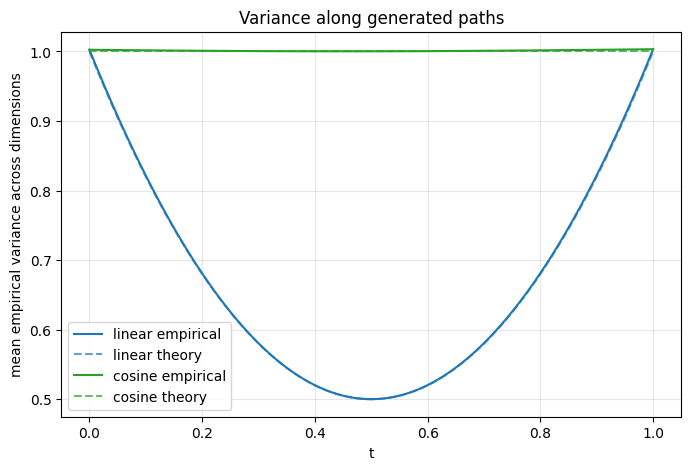
\includegraphics[width=0.78\linewidth]{figures/notebook_variance_schedules.png}
  \caption{Figure extraite du notebook : variance empirique et variance
  théorique le long des chemins linéaire et cosinus. Le schedule linéaire
  contracte la variance au milieu du transport, tandis que le schedule cosinus
  conserve l'échelle dans le cas isotrope.}
  \label{fig:variance-schedules}
\end{figure}

\section{Objectif d'apprentissage : flow matching}\label{sec:objectif-fm}

\subsection{Risque quadratique conditionnel}

Soit $T\sim\mathcal{U}([0,1])$ indépendant de $(X_0,X_1)$. On construit
$X_T=\psi_T(X_0,X_1)$ et $U_T=u_T(X_T\mid (X_0,X_1))$. On paramètre un champ de
vitesse par un réseau de neurones
\[
  v_\theta:[0,1]\times\R^d\to\R^d,
  \qquad
  (t,x)\mapsto v_\theta(t,x),
  \qquad \theta\in\R^p.
\]

\begin{definition}[Perte de flow matching conditionnel]
\[
  \boxed{
  \mathcal{L}_{\mathrm{CFM}}(\theta)
  =
  \E_{T,X_0,X_1}\left[
  \left\|v_\theta(T,X_T)-U_T\right\|_2^2
  \right].
  }
\]
\end{definition}

\subsection{Théorème de régression et équivalence des minimiseurs}

\begin{theoreme}[Minimiseur de la perte quadratique]\label{thm:regression}
Parmi toutes les fonctions mesurables $v:[0,1]\times\R^d\to\R^d$ telles que
$\E[\|v(T,X_T)\|_2^2]<\infty$, le minimiseur du risque
\[
  \mathcal{L}(v) = \E\left[\|v(T,X_T)-U_T\|_2^2\right]
\]
est, à un ensemble de mesure nulle près pour la loi de $(T,X_T)$,
\[
  v^\star(t,x) = \E[U_t\mid X_t=x] = v_t^\pi(x).
\]
\end{theoreme}

\begin{proof}
C'est la propriété classique de meilleure approximation en moyenne quadratique.
Pour une variable aléatoire $Y\in L^2$ et une tribu $\sigma(Z)$, on a, pour toute
fonction mesurable $g$ telle que $g(Z)\in L^2$,
\[
  \E\bigl[\|g(Z)-Y\|_2^2\bigr]
  =
  \E\bigl[\|g(Z)-\E[Y\mid Z]\|_2^2\bigr]
  +
  \E\bigl[\|Y-\E[Y\mid Z]\|_2^2\bigr],
\]
par le théorème de Pythagore dans $L^2(\Omega,\sigma(Z),\Prob)$ (le terme croisé
s'annule car $g(Z)-\E[Y\mid Z]$ et $Y-\E[Y\mid Z]$ sont orthogonaux : l'un est
$\sigma(Z)$-mesurable, l'autre est centré conditionnellement à $Z$). Le second
terme ne dépend pas de $g$ : le minimum en $g$ est donc atteint (et uniquement
atteint, $p_T\otimes\Law(X_T)$-presque partout) pour $g(Z)=\E[Y\mid Z]$. On
applique ceci à $Z=(T,X_T)$ et $Y=U_T$.
\end{proof}

\begin{corollaire}
En combinant le Théorème~\ref{thm:regression} et le Théorème~\ref{thm:marginalisation},
le minimiseur théorique $v_\theta^\star=v_t^\pi$ de $\mathcal{L}_{\mathrm{CFM}}$
est exactement le champ qui transporte $p_0$ vers $p_1$ au sens de l'équation de
continuité. \textbf{Minimiser une perte de régression simple sur des vitesses
conditionnelles, faciles à calculer en forme close, suffit donc à apprendre le
champ marginal qui résout le problème de transport.}
\end{corollaire}

\begin{remark}[Variance du gradient stochastique]\label{rem:variance-gradient}
La perte $\mathcal{L}_{\mathrm{CFM}}$ a le même minimiseur que la perte
\og intractable \fg{}
$\mathcal{L}(\theta)=\E_T\bigl[\int\|v_\theta(T,x)-v_T^\pi(x)\|_2^2\,p_T(x)\dd x\bigr]$,
mais son gradient stochastique a une variance différente : le choix du couplage
$\pi$ (indépendant vs. transport optimal en minibatch) influence donc la
variance de l'estimateur de gradient et la vitesse de convergence de
l'entraînement, bien que le minimiseur $\theta^\star$ reste, en théorie,
inchangé pour un réseau suffisamment expressif. C'est précisément ce levier que
la section suivante exploite.
\end{remark}

\section{Transport optimal et flow matching}\label{sec:ot-flow-matching}

Le Corollaire du Théorème~\ref{thm:regression} et le Théorème~\ref{thm:marginalisation}
montrent que \textbf{n'importe quel} couplage $\pi\in\Pi(p_0,p_1)$ donne, à la
limite de l'entraînement, un champ marginal $v_t^\pi$ qui transporte
correctement $p_0$ vers $p_1$. Mais la Remarque~\ref{rem:BB-suboptimal} a
souligné que tous les couplages ne se valent pas : le couplage indépendant
$\pi=p_0\otimes p_1$, utilisé par défaut aux Sections~\ref{sec:cfm-construction}
à~\ref{sec:objectif-fm}, ne minimise pas l'énergie cinétique du Théorème~\ref{thm:BB}, ce qui se
traduit en pratique par des trajectoires courbes et un plus grand nombre de pas
d'intégration nécessaires à la génération (Section~\ref{sec:integration-numerique}). Cette section présente
deux méthodes, de rigueur croissante, pour rapprocher le flow matching du
régime optimal caractérisé par les Théorèmes~\ref{thm:BB} et~\ref{thm:brenier}.

\subsection{Couplages par transport optimal en minibatch (OT-CFM)}

L'idée de Tong \emph{et al.} (2023, \emph{Improving and generalizing
flow-based generative models with minibatch optimal transport},
arXiv:2302.00482) est de remplacer, à chaque étape d'entraînement, l'échantillonnage
indépendant de $(X_0,X_1)$ par un échantillonnage selon une approximation
empirique du couplage optimal, calculée à l'échelle d'un minibatch.

\begin{definition}[Couplage optimal en minibatch]
Soient $x_0^{(1)},\dots,x_0^{(m)}\overset{\text{i.i.d.}}{\sim}p_0$ et
$x_1^{(1)},\dots,x_1^{(m)}\overset{\text{i.i.d.}}{\sim}p_1$ un minibatch. On
résout le problème de transport optimal discret
\[
  \widehat{P} \in \argmin_{P\in\mathcal{U}_m}\ \sum_{i,j=1}^m P_{ij}\,\bigl\|x_0^{(i)}-x_1^{(j)}\bigr\|_2^2,
  \qquad
  \mathcal{U}_m = \left\{P\in\R_+^{m\times m}\ :\ P\mathbf{1}=\frac{1}{m}\mathbf{1},\ P^\top\mathbf{1}=\frac{1}{m}\mathbf{1}\right\},
\]
par l'algorithme hongrois (coût exact, $O(m^3)$) ou par régularisation
entropique et l'algorithme de Sinkhorn (approché, $O(m^2)$ par itération). La
paire $(X_0,X_1)$ est alors tirée selon la loi discrète de matrice $\widehat{P}$
plutôt que selon le produit $p_0\otimes p_1$.
\end{definition}

On applique ensuite exactement la même perte de flow matching conditionnel
$\mathcal{L}_{\mathrm{CFM}}$ que dans la Section~\ref{sec:objectif-fm}, en tirant les paires
$(X_0,X_1)$ selon $\widehat P$ plutôt qu'indépendamment. Le
Théorème~\ref{thm:marginalisation} et le Théorème~\ref{thm:regression}
s'appliquent sans modification : quel que soit le couplage utilisé pour tirer
$(X_0,X_1)$, la perte reste valide et son minimiseur reste un champ transportant
correctement $p_0$ vers $p_1$. Seule la \emph{variance du gradient} et la
\emph{forme des trajectoires apprises} changent (Remarque~\ref{rem:variance-gradient}).

\begin{proposition}[Convergence vers le transport optimal dynamique, {Tong \emph{et al.}, 2023}]\label{prop:otcfm-convergence}
Lorsque le couplage optimal continu $\pi^\star=(\Id,T^\star)_\#p_0$ du
Théorème~\ref{thm:brenier} existe, le couplage optimal en minibatch
$\widehat P$ en constitue une approximation empirique, dont Tong \emph{et al.}
(2023) montrent qu'elle converge, lorsque la taille de minibatch $m\to\infty$,
vers le plan de transport optimal dynamique du Théorème~\ref{thm:BB}. Le champ
appris avec ce couplage (dit OT-CFM) approche donc, à taille de minibatch
suffisante, les trajectoires d'énergie cinétique minimale.
\end{proposition}

\begin{remark}
Le surcoût de calcul du couplage optimal en minibatch (résolution d'un problème
de transport de taille $m\times m$, avec $m$ la taille du minibatch, typiquement
quelques centaines) est négligeable devant le coût d'un pas de descente de
gradient sur un grand réseau, et n'intervient qu'à l'entraînement : contrairement
au CNF (Section~\ref{sec:cnf}), \textbf{aucune intégration d'ODE} n'est requise,
ni à l'entraînement ni à l'inférence. Seule la procédure d'échantillonnage des
paires $(X_0,X_1)$ change. En pratique, des trajectoires moins courbes réduisent
le nombre de pas d'intégration nécessaires lors de la génération
(Section~\ref{sec:integration-numerique}), sans en changer la nature.
\end{remark}

\subsection{Optimal Flow Matching : un flot rectiligne exact en une étape (OFM)}\label{ssec:ofm}

Le couplage OT-CFM ci-dessus n'est qu'une \emph{approximation}, de qualité
croissante avec la taille de minibatch mais jamais exacte à taille finie, et
sujette au bruit d'échantillonnage. Kornilov, Mokrov, Gasnikov et Korotin (2024,
\emph{Optimal Flow Matching: Learning Straight Trajectories in Just One Step},
arXiv:2403.13117) proposent une méthode exploitant directement le
Théorème~\ref{thm:brenier} pour retrouver, en une seule étape d'entraînement
(sans procédure itérative de \og reflow \fg{} ni heuristique de minibatch), le
couplage de Monge exact pour le coût quadratique.

\begin{definition}[Paramétrisation convexe du champ de vitesse]
On paramètre non pas directement $v_\theta$, mais un potentiel
$\varphi_\theta:\R^d\to\R$ contraint à être convexe -- par exemple à l'aide d'un
réseau à convexité garantie par construction (\emph{Input Convex Neural
Network}, Amos \emph{et al.}, 2017) -- et l'on pose
\[
  T_\theta := \nabla\varphi_\theta,
  \qquad
  X_t := (1-t)X_0 + t\,T_\theta(X_0),
  \qquad
  v_\theta(t,X_t) := T_\theta(X_0)-X_0.
\]
Le chemin est donc, par construction, le chemin linéaire du \S\,7.1
appliqué non pas à $X_1$ directement, mais à son estimation $T_\theta(X_0)$ par
le potentiel appris.
\end{definition}

\begin{theoreme}[Optimal Flow Matching, {Kornilov \emph{et al.}, 2024}]\label{thm:ofm}
Sous des hypothèses de régularité et d'expressivité suffisante de la classe des
potentiels convexes $\{\varphi_\theta\}$, le minimiseur de la perte de flow
matching conditionnel restreinte à cette paramétrisation,
\[
  \theta^\star \in \argmin_\theta\ \E_{T,X_0,X_1}\Bigl[\bigl\|\bigl(T_\theta(X_0)-X_0\bigr) - U_T\bigr\|_2^2\Bigr],
\]
vérifie $T_{\theta^\star}=T^\star$ ($p_0$-presque partout), où $T^\star=\nabla\varphi^\star$
est l'application de transport optimal du Théorème~\ref{thm:brenier}. Le flot
appris est donc, en un unique passage d'entraînement, exactement rectiligne et
de vitesse constante $U_t=T^\star(X_0)-X_0$, réalisant l'infimum du
Théorème~\ref{thm:BB}.
\end{theoreme}

\begin{remark}
On ne démontre pas ici le Théorème~\ref{thm:ofm} (voir Kornilov \emph{et al.},
2024, pour la preuve complète reposant sur la caractérisation variationnelle des
potentiels de Brenier) mais on en indique l'intuition : contraindre $T_\theta$ à
être un gradient de fonction convexe restreint drastiquement l'espace de
recherche à des applications qui \emph{peuvent} être des transports optimaux
quadratiques (par le Théorème~\ref{thm:brenier}, toute application de transport
optimal quadratique est de cette forme, et réciproquement). La perte de
régression usuelle, minimisée sur cette classe convexe plutôt que sur l'espace
de tous les champs mesurables du Théorème~\ref{thm:regression}, sélectionne
alors directement le potentiel de Brenier, sans étape itérative.
\end{remark}

\begin{corollaire}[Coût d'intégration nul]
Puisque $U_t=T^\star(X_0)-X_0$ ne dépend pas de $t$, l'ODE de génération de la
Section~\ref{sec:integration-numerique} s'intègre exactement par un unique pas d'Euler :
\[
  \widehat X_1 = \widehat X_0 + T_\theta(\widehat X_0) - \widehat X_0 = T_\theta(\widehat X_0).
\]
La génération se réduit donc à une unique évaluation du potentiel appris, sans
aucune erreur de discrétisation (Section~\ref{sec:integration-numerique}).
\end{corollaire}

\begin{center}
\small
\renewcommand{\arraystretch}{1.4}
\begin{tabular}{@{}p{2.8cm}p{4.0cm}p{3.8cm}p{2.7cm}@{}}
\toprule
\textbf{Méthode} & \textbf{Couplage} & \textbf{Coût entraînement} & \textbf{Pas à l'inférence} \\
\midrule
CFM (couplage indépendant) & $\pi=p_0\otimes p_1$ & régression, simulation-free & $N\gg 1$ (trajectoires courbes) \\
OT-CFM (Tong \emph{et al.}, 2023) & OT discret en minibatch, approché & régression + OT $m\times m$ par batch & $N$ réduit \\
OFM (Kornilov \emph{et al.}, 2024) & OT exact (Brenier), sous hypothèses & régression sur potentiel convexe & $N=1$ exact \\
\bottomrule
\end{tabular}
\end{center}

\section{Génération par intégration numérique}\label{sec:integration-numerique}

\subsection{ODE de génération et erreur de discrétisation}

Après entraînement, on remplace le champ exact $v_t^\pi$ par son approximation
$v_\theta(t,x)$. Pour générer, on échantillonne $\widehat X_0\sim p_0$ puis on
résout
\[
  \frac{\dd \widehat X_t}{\dd t} = v_\theta(t,\widehat X_t),
  \qquad \widehat X_{t=0}\sim p_0.
\]
La sortie générée est $\widehat X_1$.

\begin{definition}[Schéma d'Euler explicite]
Avec $N\in\N^\star$ pas et $\Delta t = 1/N$, $t_k=k/N$ pour $k=0,\dots,N-1$ :
\[
  \widehat X_{k+1} = \widehat X_k + \Delta t\,v_\theta(t_k,\widehat X_k).
\]
\end{definition}

\begin{proposition}[Ordre de convergence d'Euler]
Si $v_\theta$ est lipschitzienne en $x$ (constante $L$) uniformément en $t$, et
de classe $\mathcal{C}^1$ en $t$, l'erreur globale du schéma d'Euler explicite
après $N$ pas vérifie
\[
  \max_{0\le k\le N}\|\widehat X_k - X_{t_k}\|_2 = O(\Delta t) = O(1/N),
\]
c'est-à-dire que le schéma d'Euler est d'ordre $1$ (l'erreur locale par pas est
en $O(\Delta t^2)$, l'accumulation sur $N=1/\Delta t$ pas donne une erreur
globale en $O(\Delta t)$).
\end{proposition}

\begin{remark}
Des schémas d'ordre supérieur (Heun / RK2, en $O(\Delta t^2)$ globalement, ou
Runge--Kutta d'ordre $4$, en $O(\Delta t^4)$) permettent de réduire fortement le
nombre de pas nécessaires pour une précision donnée, au prix d'évaluations
supplémentaires de $v_\theta$ par pas. Le schéma de Heun s'écrit
\[
  \widetilde X_{k+1} = \widehat X_k + \Delta t\, v_\theta(t_k,\widehat X_k),
  \qquad
  \widehat X_{k+1} = \widehat X_k + \frac{\Delta t}{2}\Bigl(v_\theta(t_k,\widehat X_k)+v_\theta(t_{k+1},\widetilde X_{k+1})\Bigr).
\]
\end{remark}

\begin{lstlisting}[style=pythoncourse,caption={Simulation Euler d'un flow appris}]
@torch.no_grad()
def sample_flow(model, n_samples, n_steps, shape, device):
    x = torch.randn(n_samples, *shape, device=device)
    dt = 1.0 / n_steps

    model.eval()
    for k in range(n_steps):
        t = torch.full((n_samples,), k / n_steps, device=device)
        velocity = model(x, t)
        x = x + dt * velocity

    return x
\end{lstlisting}

Dans ce code, l'appel \texttt{model(x, t)} correspond mathématiquement à
$v_\theta(t,x)$ ; l'ordre des arguments est seulement une convention
d'implémentation.

\begin{lstlisting}[style=pythoncourse,caption={Schéma de Heun (ordre 2)}]
@torch.no_grad()
def sample_flow_heun(model, n_samples, n_steps, shape, device):
    x = torch.randn(n_samples, *shape, device=device)
    dt = 1.0 / n_steps

    model.eval()
    for k in range(n_steps):
        t0 = torch.full((n_samples,), k / n_steps, device=device)
        t1 = torch.full((n_samples,), (k + 1) / n_steps, device=device)

        v0 = model(x, t0)
        x_pred = x + dt * v0
        v1 = model(x_pred, t1)

        x = x + 0.5 * dt * (v0 + v1)

    return x
\end{lstlisting}

\section{Exemple 1 : distribution 2D \texttt{make\_moons}}

\subsection{Construction du dataset}

On veut apprendre à transformer un bruit gaussien 2D en une distribution en
forme de deux lunes :
\[
  X_0 \sim \mathcal{N}(0,I_2),
  \qquad
  X_1 \sim p_{\mathrm{moons}},
\]
où $p_{\mathrm{moons}}$ désigne la loi empirique des points du dataset
\texttt{make\_moons}, avec couplage indépendant $\pi=p_0\otimes p_{\mathrm{moons}}$.
On utilise le chemin cosinus (\S\,7.2) :
\[
  X_t = \cos\Bigl(\frac{\pi}{2}t\Bigr)X_0 + \sin\Bigl(\frac{\pi}{2}t\Bigr)X_1,
  \qquad
  U_t = -\frac{\pi}{2}\sin\Bigl(\frac{\pi}{2}t\Bigr)X_0 + \frac{\pi}{2}\cos\Bigl(\frac{\pi}{2}t\Bigr)X_1.
\]

\subsection{Code minimal}

\begin{lstlisting}[style=pythoncourse,caption={Interpolation cosinus et cible de vitesse}]
def cosine_schedule_torch(t):
    c = torch.pi / 2.0
    alpha = torch.cos(c * t)
    beta = torch.sin(c * t)
    d_alpha = -c * torch.sin(c * t)
    d_beta = c * torch.cos(c * t)
    return alpha, beta, d_alpha, d_beta

x0 = torch.randn(n_train, 2, device=device)
x1 = moons_torch[torch.randint(0, len(moons_torch), (n_train,), device=device)]
t = torch.rand(n_train, 1, device=device)

alpha, beta, d_alpha, d_beta = cosine_schedule_torch(t)
xt = alpha * x0 + beta * x1
target_velocity = d_alpha * x0 + d_beta * x1
\end{lstlisting}

Le modèle est un MLP recevant les features $(x_t,\,t,\,\sin(\pi t),\,\cos(\pi t))$,
où $x_t\in\R^2$ est une réalisation de $X_t$ ; le modèle prédit une vitesse dans
$\R^2$, cible de la régression du Théorème~\ref{thm:regression}.

\begin{lstlisting}[style=pythoncourse,caption={Loss de flow matching pour l'exemple 2D}]
features = model_features_torch(xt, t)
pred_velocity = flow_model(features)
loss = F.mse_loss(pred_velocity, target_velocity)
\end{lstlisting}

\subsection{Schéma du modèle et sortie du notebook}

\begin{figure}[htbp]
  \centering
  \resizebox{\linewidth}{!}{%
  \begin{tikzpicture}[node distance=8mm]
    \node[modelblock] (in) {$x_t\in\R^2$\\$t,\sin(\pi t),\cos(\pi t)$\\features $=5$};
    \node[modelop, right=of in] (std) {standardisation\\entrée};
    \node[modelblock, right=of std] (l1) {Linear\\$5\to256$\\SiLU};
    \node[modelblock, right=of l1] (l2) {Linear\\$256\to256$\\SiLU};
    \node[modelblock, right=of l2] (l3) {Linear\\$256\to256$\\SiLU};
    \node[modelblock, right=of l3] (out) {Linear\\$256\to2$};
    \node[modelop, right=of out] (destd) {déstandardisation\\sortie};
    \node[modelblock, right=of destd] (vel) {$v_\theta(t,x_t)\in\R^2$};

    \draw[modelarrow] (in) -- (std);
    \draw[modelarrow] (std) -- (l1);
    \draw[modelarrow] (l1) -- (l2);
    \draw[modelarrow] (l2) -- (l3);
    \draw[modelarrow] (l3) -- (out);
    \draw[modelarrow] (out) -- (destd);
    \draw[modelarrow] (destd) -- (vel);
  \end{tikzpicture}}
  \caption{Schéma du MLP utilisé dans le notebook pour l'expérience
  \texttt{make\_moons}. Le réseau prédit une vitesse 2D à partir de la position
  courante et d'un encodage temporel trigonométrique.}
  \label{fig:mlp-schema}
\end{figure}

\begin{figure}[htbp]
  \centering
  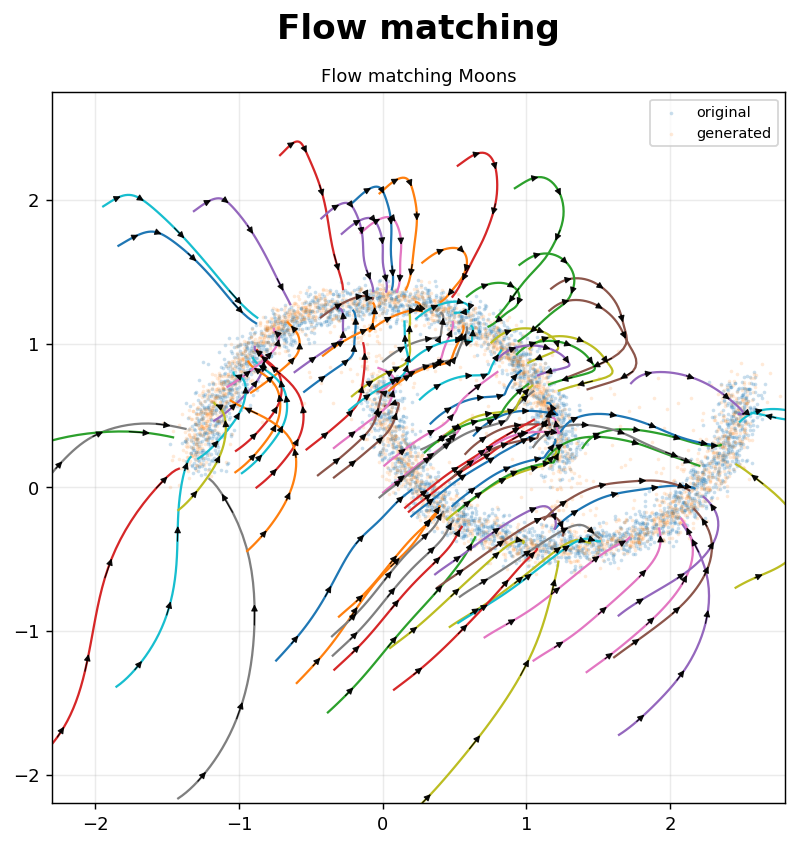
\includegraphics[width=0.86\linewidth]{figures/notebook_flow_matching_moons.png}
  \caption{Figure extraite du notebook : distribution \texttt{make\_moons},
  échantillons générés et trajectoires obtenues en intégrant le champ de vitesse
  appris par Euler.}
  \label{fig:moons-notebook}
\end{figure}

\subsection{Variante OT-CFM sur \texttt{make\_moons} : comparaison des vecteurs}

Dans l'expérience précédente, le couplage utilisé est indépendant :
\[
  (X_0,X_1)\sim p_0\otimes p_{\mathrm{moons}}.
\]
Les paires bruit--donnée sont donc arbitraires. Cela peut produire des vecteurs
conditionnels longs et désordonnés, notamment pour le chemin linéaire
$U_t=X_1-X_0$.

La variante OT-CFM remplace ce couplage indépendant par un couplage optimal
\emph{dans chaque minibatch}. Si le batch source est
$\{x_0^{(i)}\}_{i=1}^m$ et le batch cible est $\{x_1^{(j)}\}_{j=1}^m$, on construit
la matrice de coûts
\[
  C_{ij}=\|x_0^{(i)}-x_1^{(j)}\|_2^2.
\]
On cherche ensuite la permutation optimale
\[
  \sigma^\star
  =
  \argmin_{\sigma\in\mathfrak{S}_m}
  \sum_{i=1}^m C_{i,\sigma(i)}.
\]
Le batch d'entraînement devient alors
\[
  \bigl(x_0^{(i)},x_1^{(\sigma^\star(i))}\bigr)_{i=1}^m.
\]
Pour le schedule linéaire, les vitesses cibles comparées sont donc
\[
  u_{\mathrm{ind}}^{(i)}=x_{1,\mathrm{ind}}^{(i)}-x_0^{(i)},
  \qquad
  u_{\mathrm{OT}}^{(i)}=x_1^{(\sigma^\star(i))}-x_0^{(i)}.
\]

\begin{lstlisting}[style=pythoncourse,caption={Matching OT minibatch pour make\_moons}]
from scipy.optimize import linear_sum_assignment

def minibatch_ot_pairs(x0, x1):
    # x0: (m, d), x1: (m, d)
    cost = ((x0[:, None, :] - x1[None, :, :]) ** 2).sum(axis=-1)
    row_ind, col_ind = linear_sum_assignment(cost)
    x1_ot = x1[col_ind]
    return x0[row_ind], x1_ot

x0_ot, x1_ot = minibatch_ot_pairs(x0_batch, x1_batch)
target_velocity_ot = x1_ot - x0_ot
\end{lstlisting}

\begin{figure}[htbp]
  \centering
  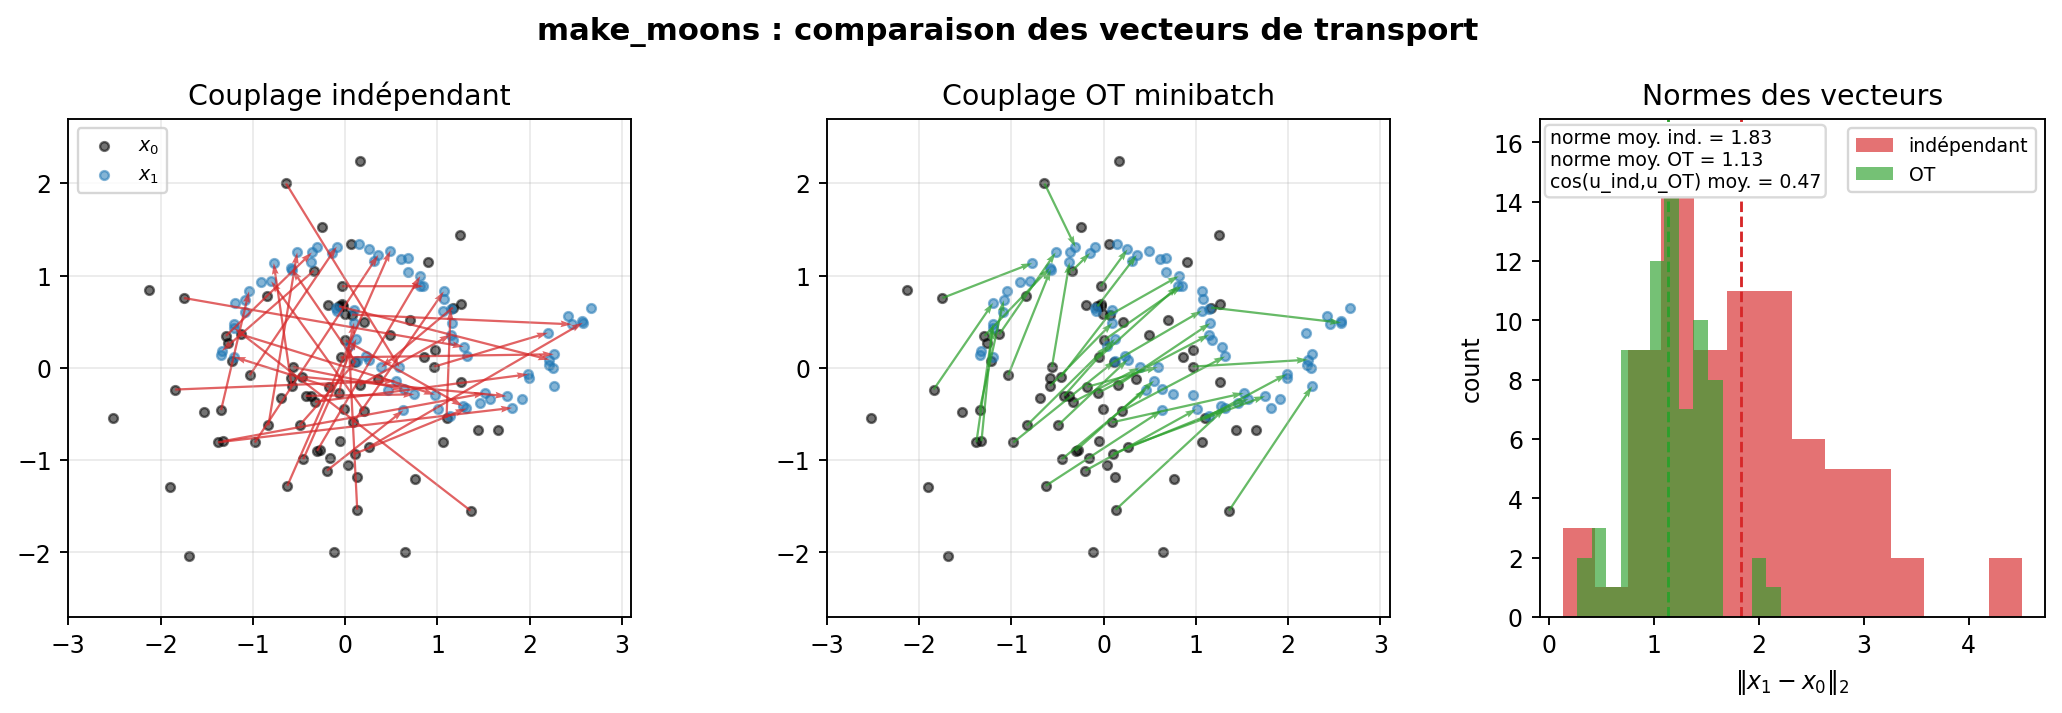
\includegraphics[width=\linewidth]{figures/ot_moons_vector_comparison.png}
  \caption{Comparaison pratique sur \texttt{make\_moons}. À gauche, le couplage
  indépendant produit des vecteurs plus longs et plus croisés. Au centre, le
  couplage OT en minibatch associe chaque bruit à une cible plus proche au sens
  quadratique. À droite, les normes $\|x_1-x_0\|_2$ montrent que l'OT réduit
  l'énergie cinétique moyenne du transport.}
  \label{fig:ot-moons-vectors}
\end{figure}

\section{Exemple 2 : MNIST avec U-Net}

\subsection{Passage aux images}

Pour MNIST, chaque image est un tenseur $x_1\in\R^{1\times 28\times 28}$,
réalisation de $X_1\sim p_{\mathrm{data}}$. On choisit un bruit
$X_0\sim\mathcal{N}(0,I_d)$, $d=1\cdot28\cdot28$, de même taille que l'image. Le
réseau doit prédire une vitesse image $v_\theta(t,x_t)\in\R^{1\times 28\times 28}$.
Comme la sortie a la même taille que l'entrée, un U-Net est naturel : il combine
des features locales et globales, puis reconstruit une image de vitesse, en
approximant $v_t^\pi(x)=\E[U_t\mid X_t=x]$ (Théorèmes~\ref{thm:marginalisation}
et~\ref{thm:regression}).

\subsection{Interpolation utilisée}

\begin{lstlisting}[style=pythoncourse,caption={Interpolation linéaire ou cosinus pour MNIST}]
def interpolate_flow(x0, x1, t, interpolation="linear"):
    t_view = t.view(-1, 1, 1, 1)

    if interpolation == "linear":
        xt = (1 - t_view) * x0 + t_view * x1
        target_velocity = x1 - x0

    elif interpolation == "cos":
        angle = torch.pi * t_view / 2
        alpha = torch.cos(angle)
        beta = torch.sin(angle)
        d_alpha = -(torch.pi / 2) * torch.sin(angle)
        d_beta = (torch.pi / 2) * torch.cos(angle)

        xt = alpha * x0 + beta * x1
        target_velocity = d_alpha * x0 + d_beta * x1

    return xt, target_velocity
\end{lstlisting}

\subsection{Boucle d'entraînement}

\begin{lstlisting}[style=pythoncourse,caption={Étape d'entraînement flow matching sur MNIST}]
for x1, _ in train_loader:
    x1 = x1.to(device)
    x1 = x1 * 2 - 1

    x0 = torch.randn_like(x1)
    t = torch.rand(x1.shape[0], device=device)

    xt, target_velocity = interpolate_flow(x0, x1, t, interpolation="cos")
    pred_velocity = model(xt, t)

    loss = F.mse_loss(pred_velocity, target_velocity)
    optimizer.zero_grad(set_to_none=True)
    loss.backward()
    optimizer.step()
\end{lstlisting}

\subsection{Schéma du U-Net et sortie du notebook}

\begin{figure}[htbp]
  \centering
  \resizebox{\linewidth}{!}{%
  \begin{tikzpicture}[node distance=7mm]
    \node[modelblock] (input) {$x_t$\\$1\times28\times28$};
    \node[modelop, right=of input] (concat) {concaténation\\carte temps $t$\\$2\times28\times28$};
    \node[modelblock, right=of concat] (enc1) {Enc1\\DoubleConv\\$2\to32$\\$28\times28$};
    \node[modelop, right=of enc1] (pool1) {MaxPool\\$28\to14$};
    \node[modelblock, right=of pool1] (enc2) {Enc2\\DoubleConv\\$32\to64$\\$14\times14$};
    \node[modelop, right=of enc2] (pool2) {MaxPool\\$14\to7$};
    \node[modelblock, right=of pool2] (bottleneck) {Bottleneck\\DoubleConv\\$64\to64$\\$7\times7$};

    \node[modelop, below=13mm of bottleneck] (up1) {ConvTranspose\\$7\to14$\\$64\to64$};
    \node[modelblock, left=of up1] (dec1) {Dec1\\skip Enc2\\DoubleConv\\$64\to32$\\$14\times14$};
    \node[modelop, left=of dec1] (up2) {ConvTranspose\\$14\to28$\\$32\to32$};
    \node[modelblock, left=of up2] (dec2) {Dec2\\skip Enc1\\DoubleConv\\$32\to32$\\$28\times28$};
    \node[modelblock, left=of dec2] (out) {Conv $1\times1$\\$32\to1$\\$v_\theta(t,x_t)$};

    \draw[modelarrow] (input) -- (concat);
    \draw[modelarrow] (concat) -- (enc1);
    \draw[modelarrow] (enc1) -- (pool1);
    \draw[modelarrow] (pool1) -- (enc2);
    \draw[modelarrow] (enc2) -- (pool2);
    \draw[modelarrow] (pool2) -- (bottleneck);
    \draw[modelarrow] (bottleneck) -- (up1);
    \draw[modelarrow] (up1) -- (dec1);
    \draw[modelarrow] (dec1) -- (up2);
    \draw[modelarrow] (up2) -- (dec2);
    \draw[modelarrow] (dec2) -- (out);
    \draw[modelskip] (enc2.south) to[out=-90,in=90] (dec1.north);
    \draw[modelskip] (enc1.south) to[out=-90,in=90] (dec2.north);
  \end{tikzpicture}}
  \caption{Schéma du U-Net utilisé dans le notebook. Chaque bloc
  \texttt{DoubleConv} correspond à deux convolutions $3\times3$ suivies de ReLU.
  Le temps $t$ est injecté comme une carte constante concaténée à l'image bruitée
  $x_t$.}
  \label{fig:unet-schema}
\end{figure}

\begin{figure}[htbp]
  \centering
  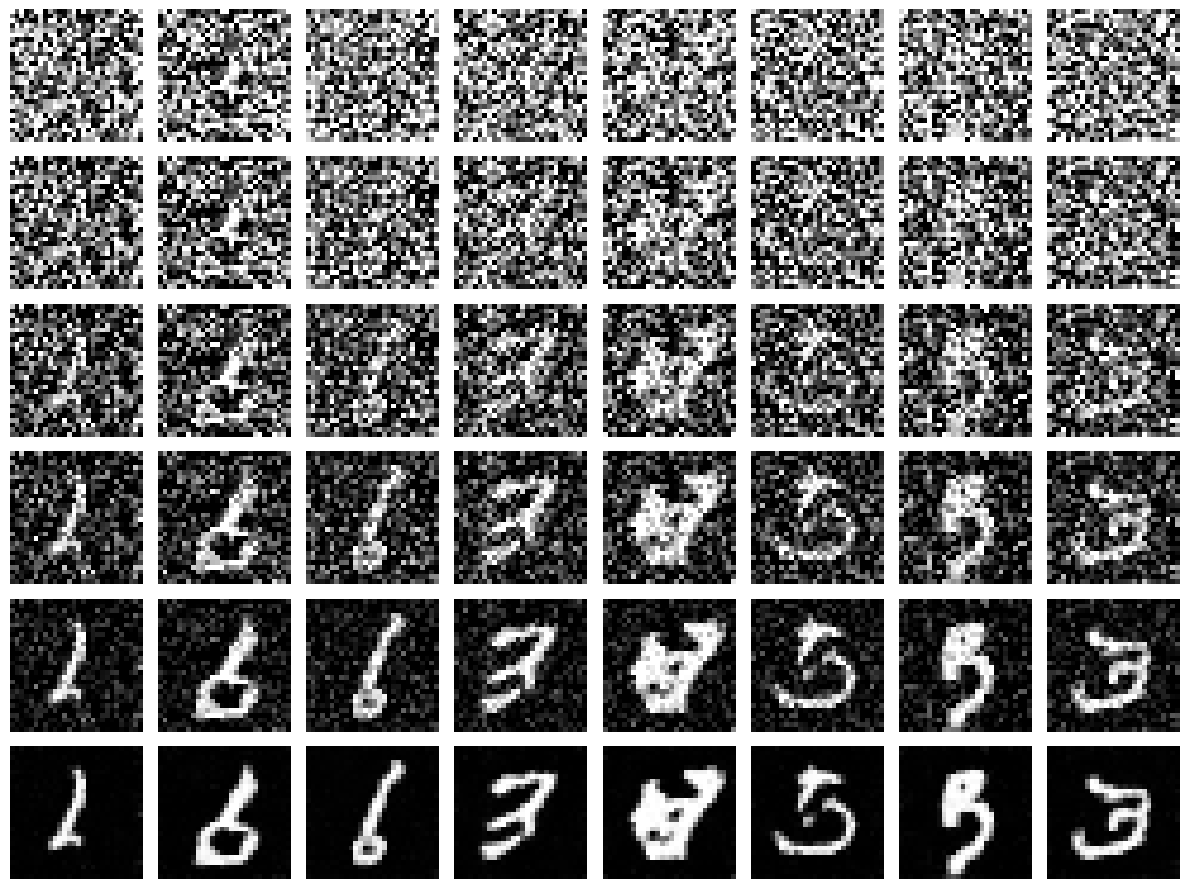
\includegraphics[width=0.92\linewidth]{figures/notebook_mnist_trajectory.png}
  \caption{Figure extraite du notebook : évolution de plusieurs échantillons
  MNIST pendant l'intégration de l'ODE apprise. Les lignes correspondent à des
  instants de simulation successifs.}
  \label{fig:mnist-notebook}
\end{figure}

\subsection{Variante OT-CFM sur MNIST : comparaison des vecteurs en espace image}

Pour les images, le même principe s'applique après vectorisation :
\[
  x_0^{(i)},x_1^{(j)}\in\R^{784},
  \qquad
  C_{ij}=\|x_0^{(i)}-x_1^{(j)}\|_2^2.
\]
On résout à chaque batch un problème d'affectation optimal entre les bruits et
les images du batch. Le vecteur de transport est alors une image de même taille
que MNIST :
\[
  u^{(i)} = x_1^{(\sigma^\star(i))}-x_0^{(i)}
  \in \R^{1\times 28\times 28}.
\]
On peut visualiser ce vecteur pixel par pixel avec une colormap signée :
les zones rouges correspondent aux pixels que le champ doit augmenter, les zones
bleues aux pixels qu'il doit diminuer.

\begin{lstlisting}[style=pythoncourse,caption={OT-CFM en espace pixel pour MNIST}]
from scipy.optimize import linear_sum_assignment

def minibatch_ot_images(x0, x1):
    # x0, x1: (m, 1, 28, 28), valeurs dans [-1, 1]
    m = x0.shape[0]
    x0_flat = x0.reshape(m, -1)
    x1_flat = x1.reshape(m, -1)
    cost = ((x0_flat[:, None, :] - x1_flat[None, :, :]) ** 2).sum(axis=-1)
    row_ind, col_ind = linear_sum_assignment(cost)
    return x0[row_ind], x1[col_ind]

x0_ot, x1_ot = minibatch_ot_images(x0_batch, x1_batch)
xt, target_velocity = interpolate_flow(x0_ot, x1_ot, t, interpolation="cos")
\end{lstlisting}

\begin{warningbox}
Pour MNIST, cette procédure réalise un transport optimal dans l'espace pixel
$\R^{784}$. Elle minimise bien une distance quadratique entre tenseurs, mais ce
n'est pas nécessairement une distance sémantique entre chiffres. Deux images
visuellement proches pour un humain peuvent être éloignées en norme pixel, et
réciproquement. Pour améliorer ce point, on peut calculer l'OT dans un espace de
features appris plutôt que directement dans l'espace image.
\end{warningbox}

\begin{figure}[htbp]
  \centering
  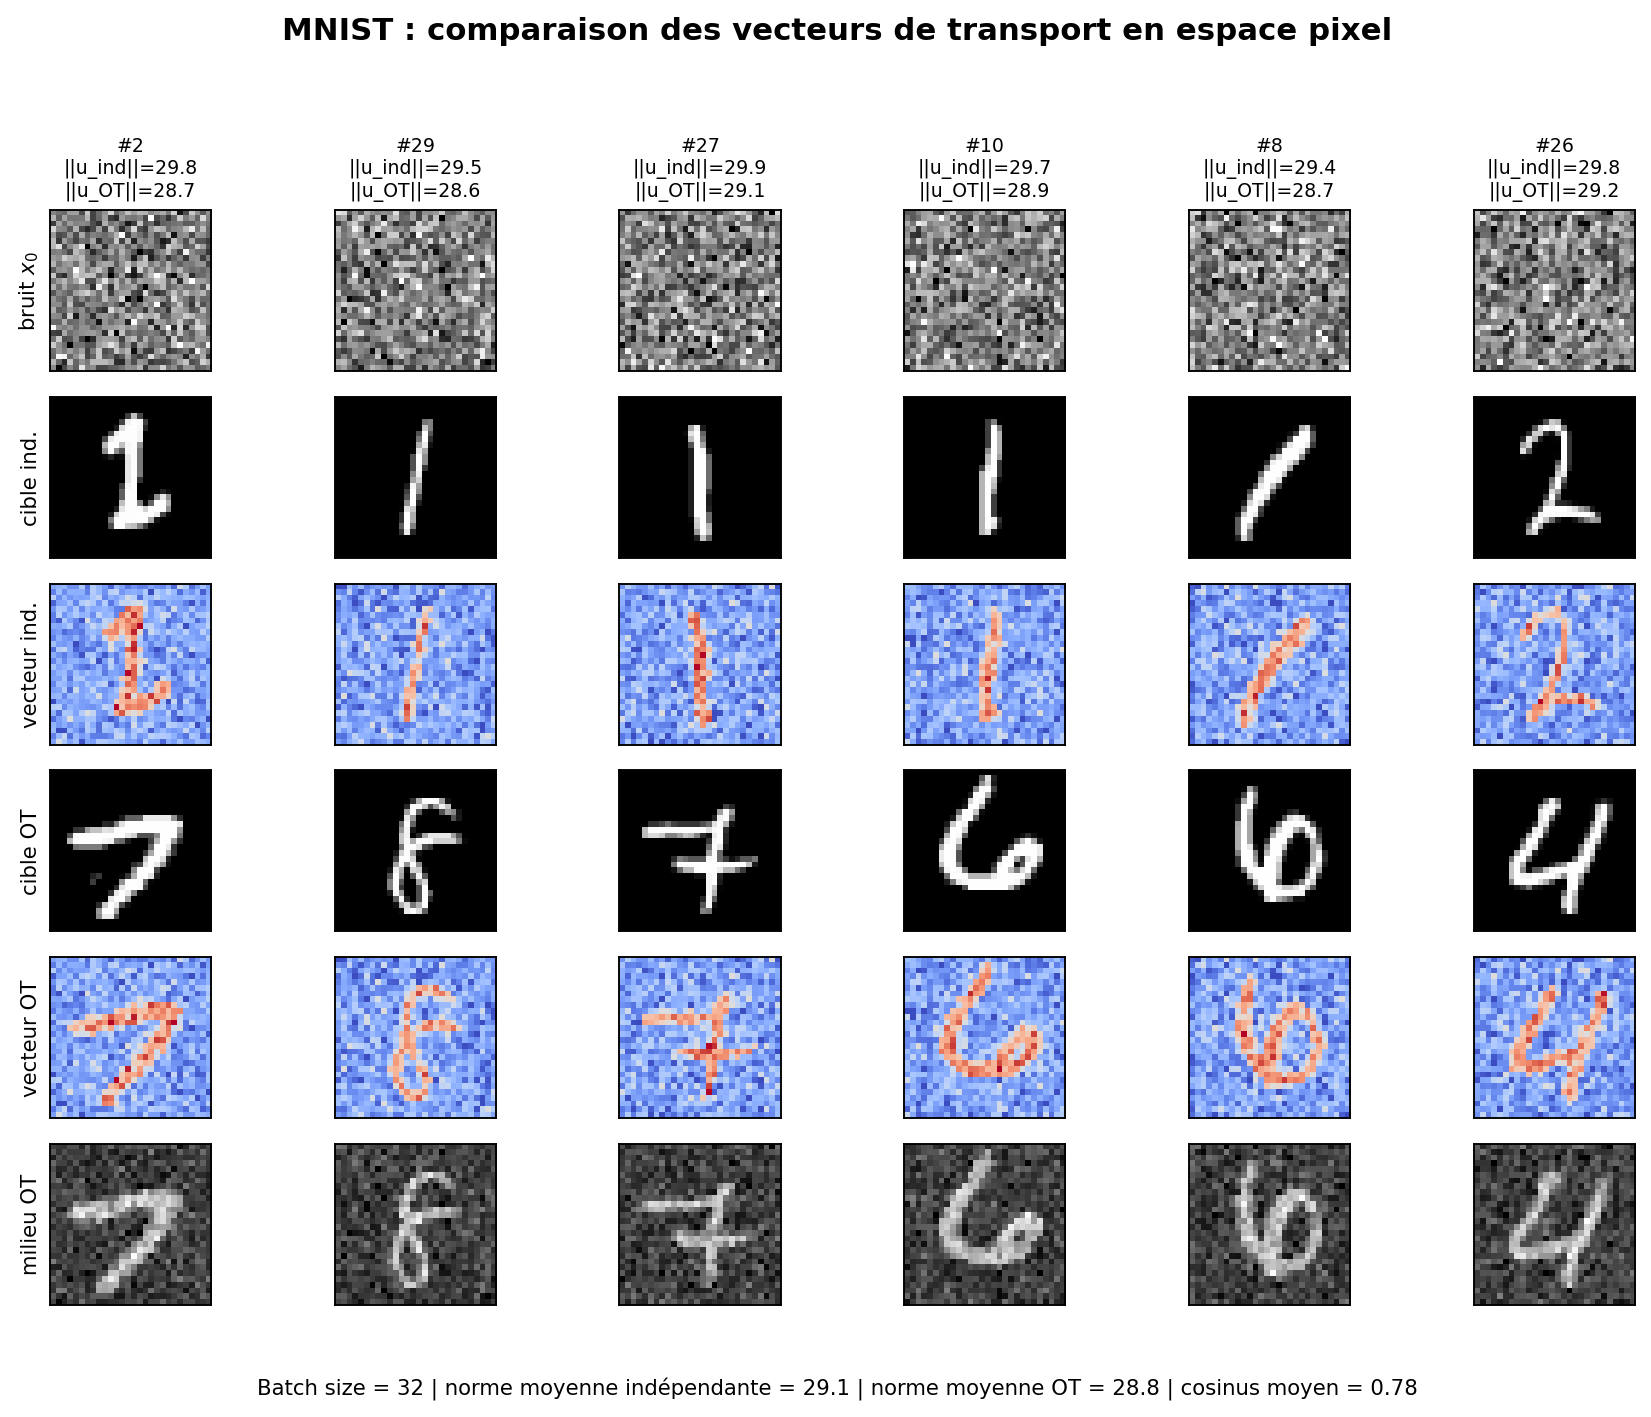
\includegraphics[width=0.92\linewidth]{figures/ot_mnist_vector_comparison.png}
  \caption{Comparaison MNIST en espace pixel. Chaque colonne fixe un bruit
  $x_0$. Les lignes comparent la cible issue d'un couplage indépendant, le
  vecteur indépendant, la cible issue du matching OT, le vecteur OT, puis le
  milieu de trajectoire OT. Les normes affichées montrent que l'OT réduit en
  général la longueur du vecteur de transport, mais la correspondance reste
  définie par une distance pixel.}
  \label{fig:ot-mnist-vectors}
\end{figure}

\section{Comparaison expérimentale : CFM contre OT-CFM}\label{sec:comparaison-experimentale}

Les sections précédentes ont entraîné, sur \texttt{make\_moons} et sur MNIST, un flow matching
classique (CFM, couplage indépendant $\pi=p_0\otimes p_1$) et comparé \emph{ponctuellement} les
vecteurs de transport obtenus avec un couplage OT en minibatch
(Figures~\ref{fig:ot-moons-vectors} et~\ref{fig:ot-mnist-vectors}). Cette section va plus loin :
on entraîne un \emph{second} modèle complet avec la perte OT-CFM (couplage optimal en minibatch à
chaque itération, Section~\ref{sec:ot-flow-matching}) sur les deux mêmes jeux de données, et on
compare les deux modèles \emph{entraînés} -- pas seulement les vecteurs de couplage -- sur la
rectitude des trajectoires, l'énergie cinétique et la qualité de génération en fonction du nombre
de pas d'intégration. Le code complet se trouve dans \texttt{ot\_flow\_matching.ipynb}.

\begin{warningbox}
Pour isoler l'effet du couplage (et non celui de la forme du chemin conditionnel), les deux
modèles de cette section utilisent le \textbf{schedule linéaire} $X_t=(1-t)X_0+tX_1$,
$U_t=X_1-X_0$ (\S\,7.1), et non le schedule cosinus utilisé dans \texttt{notebook.ipynb}. C'est
uniquement avec un chemin conditionnel déjà rectiligne que le couplage OT peut produire des
trajectoires \emph{marginales} rectilignes (Théorème~\ref{thm:brenier} et remarque suivante) : avec
un chemin courbe, comparer les deux couplages mélangerait deux effets géométriques distincts et
rendrait la comparaison ininterprétable.
\end{warningbox}

\subsection{Rectitude des trajectoires et énergie cinétique sur \texttt{make\_moons}}

Les deux modèles (MLP identique, \S\,10.2) sont entraînés $4000$ itérations chacun, puis on simule
$600$ trajectoires par intégration d'Euler à $N=100$ pas, à partir des \emph{mêmes} points de bruit
$X_0$ pour les deux modèles.

\begin{figure}[htbp]
  \centering
  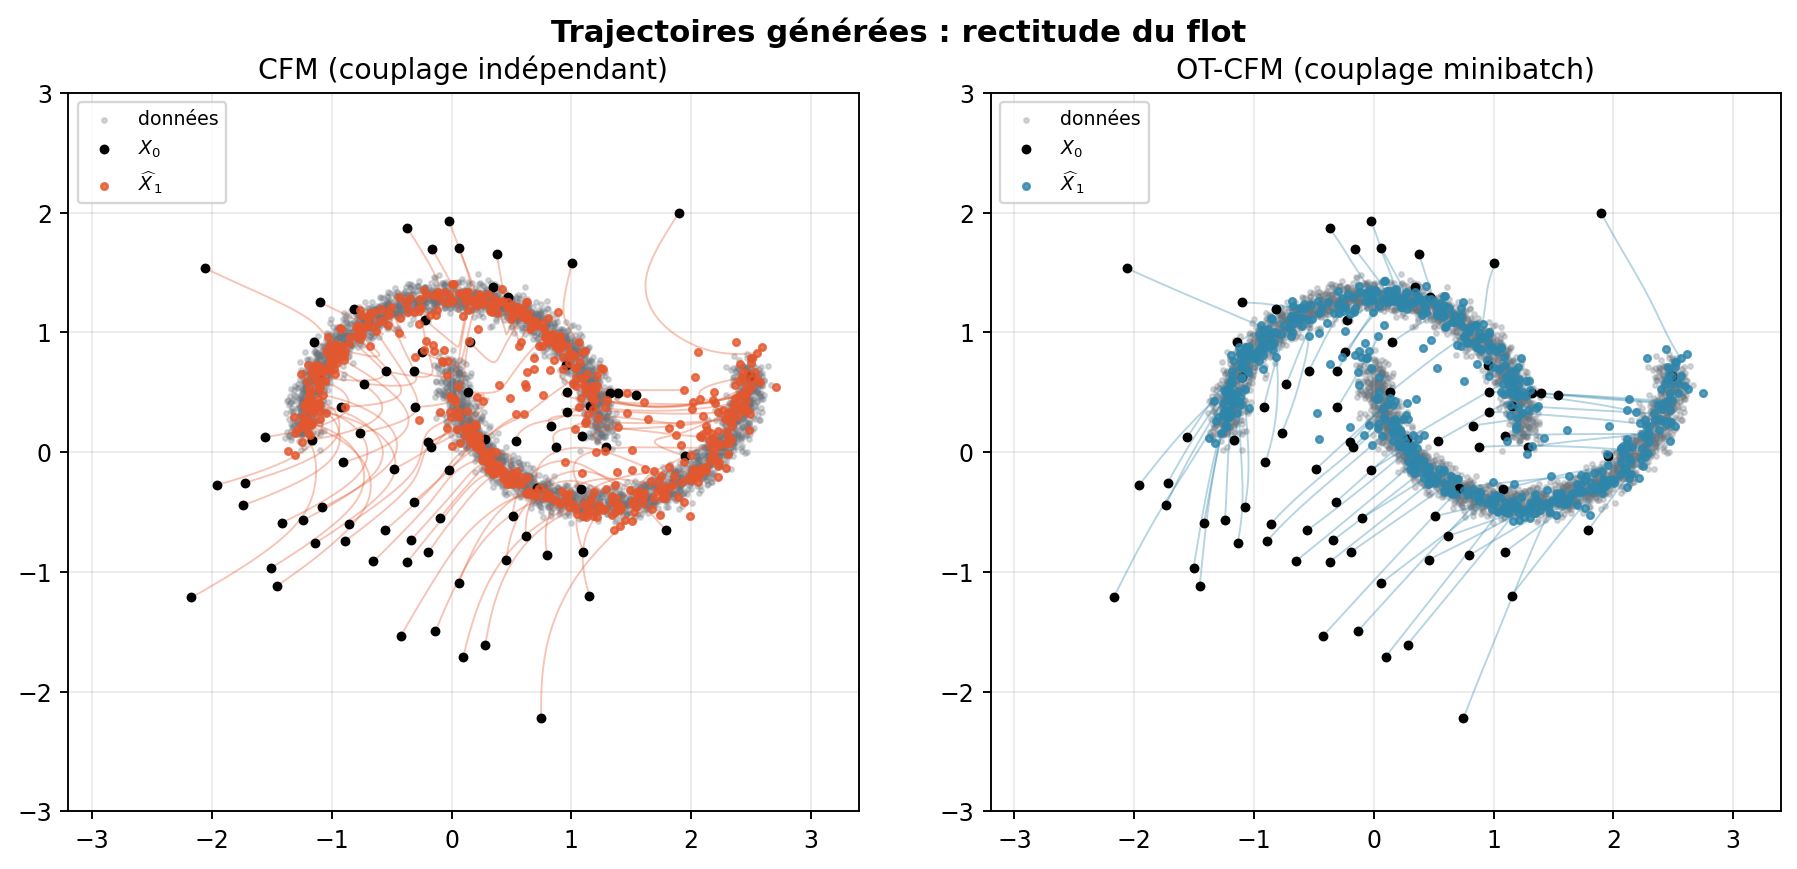
\includegraphics[width=\linewidth]{figures/cfm_vs_otcfm_moons_trajectories.png}
  \caption{Trajectoires générées par le modèle CFM (gauche) et le modèle OT-CFM (droite), à partir
  des mêmes échantillons de bruit. Les trajectoires OT-CFM sont visiblement quasi rectilignes,
  contrairement aux trajectoires CFM qui contournent la masse de probabilité.}
  \label{fig:cfm-otcfm-moons-traj}
\end{figure}

Pour quantifier cette différence, on mesure, pour chaque trajectoire, l'écart quadratique moyen
au segment $[\widehat X_0,\widehat X_1]$ (\og rectitude \fg{}), et l'énergie cinétique moyenne
$\int_0^1\E[\|v_\theta(t,X_t)\|_2^2]\dd t$ (approximation par somme de Riemann le long des
trajectoires simulées, cf. Théorème~\ref{thm:BB}).

\begin{figure}[htbp]
  \centering
  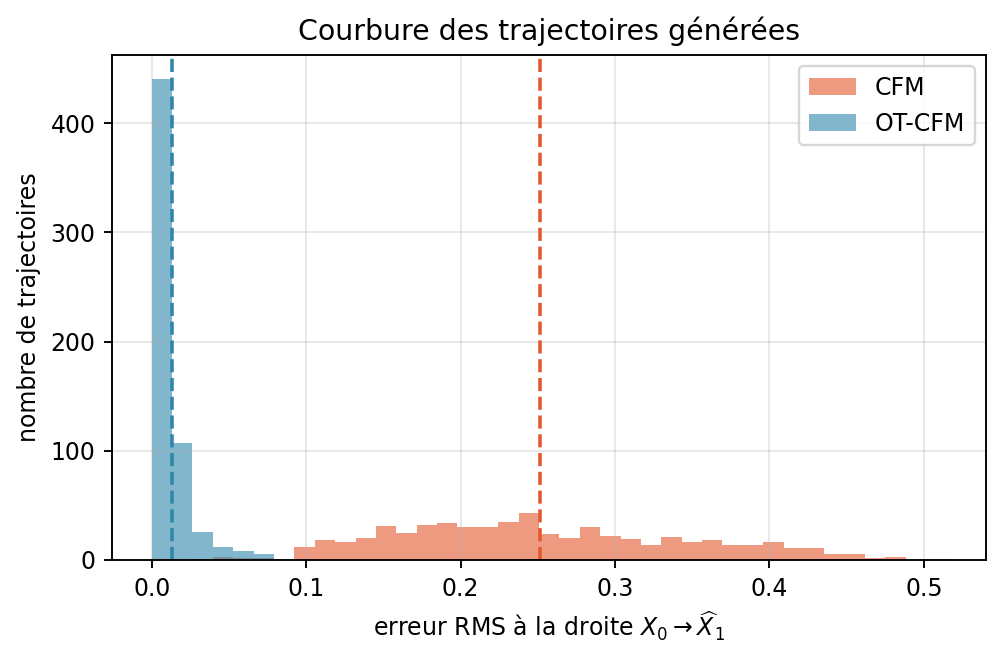
\includegraphics[width=0.7\linewidth]{figures/cfm_vs_otcfm_straightness.png}
  \caption{Distribution de l'erreur de rectitude (écart RMS à la droite $\widehat X_0\to\widehat
  X_1$) pour les $600$ trajectoires générées par chaque modèle.}
  \label{fig:cfm-otcfm-straightness}
\end{figure}

Sur cette expérience, l'erreur de rectitude moyenne passe de $0{,}251$ (CFM) à $0{,}013$ (OT-CFM),
et l'énergie cinétique moyenne de $1{,}80$ à $1{,}02$, soit une réduction de $43\%$ -- cohérent avec
le Théorème~\ref{thm:BB} : le couplage optimal en minibatch rapproche l'énergie cinétique du
transport de la borne inférieure donnée par $W_2(p_0,p_1)^2$.

\subsection{Qualité de génération en fonction du nombre de pas (NFE)}

Une conséquence pratique directe de la rectitude : moins de pas d'intégration suffisent pour
approcher la distribution cible. On mesure la distance de Wasserstein empirique $\widehat W_2$
(coût quadratique, calculée exactement entre deux échantillons de même taille par affectation
optimale, comme au \S\,\ref{sec:ot-flow-matching}) entre les échantillons générés et
\texttt{make\_moons}, pour un nombre de pas $N$ croissant.

\begin{figure}[htbp]
  \centering
  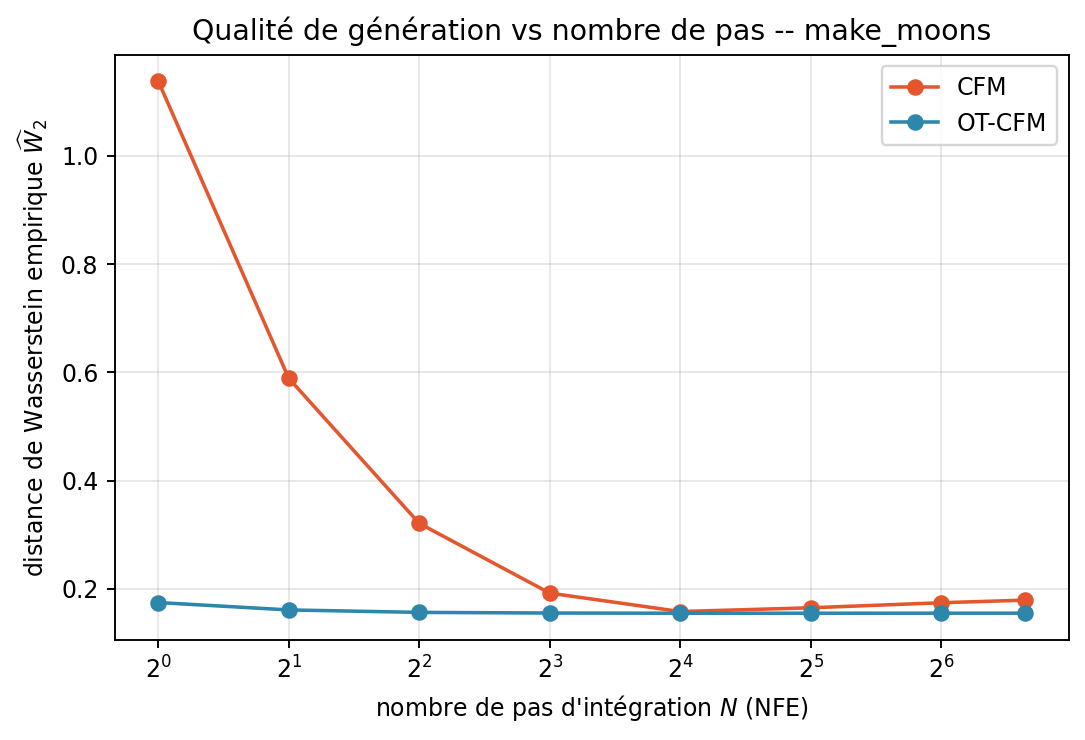
\includegraphics[width=0.72\linewidth]{figures/cfm_vs_otcfm_nfe_quality.png}
  \caption{Distance de Wasserstein empirique $\widehat W_2$ entre échantillons générés et données,
  en fonction du nombre de pas d'intégration $N$ (échelle log). Le modèle OT-CFM atteint sa qualité
  asymptotique dès $N=1$ à $2$ pas, tandis que le modèle CFM nécessite $N\gtrsim 16$ pas pour
  converger au même niveau.}
  \label{fig:cfm-otcfm-nfe}
\end{figure}

À $N=1$ pas (un unique pas d'Euler, c'est-à-dire $\widehat X_1=\widehat X_0+v_\theta(0,\widehat
X_0)$), le modèle OT-CFM atteint déjà $\widehat W_2\approx 0{,}17$, contre $\widehat W_2\approx
1{,}13$ pour le modèle CFM : à couplage optimal, une trajectoire quasi rectiligne se prête bien à
une intégration en très peu de pas, alors qu'une trajectoire courbe nécessite de nombreux petits
pas pour suivre correctement sa courbure (erreur d'Euler en $O(\Delta t)$,
Section~\ref{sec:integration-numerique}).

\begin{figure}[htbp]
  \centering
  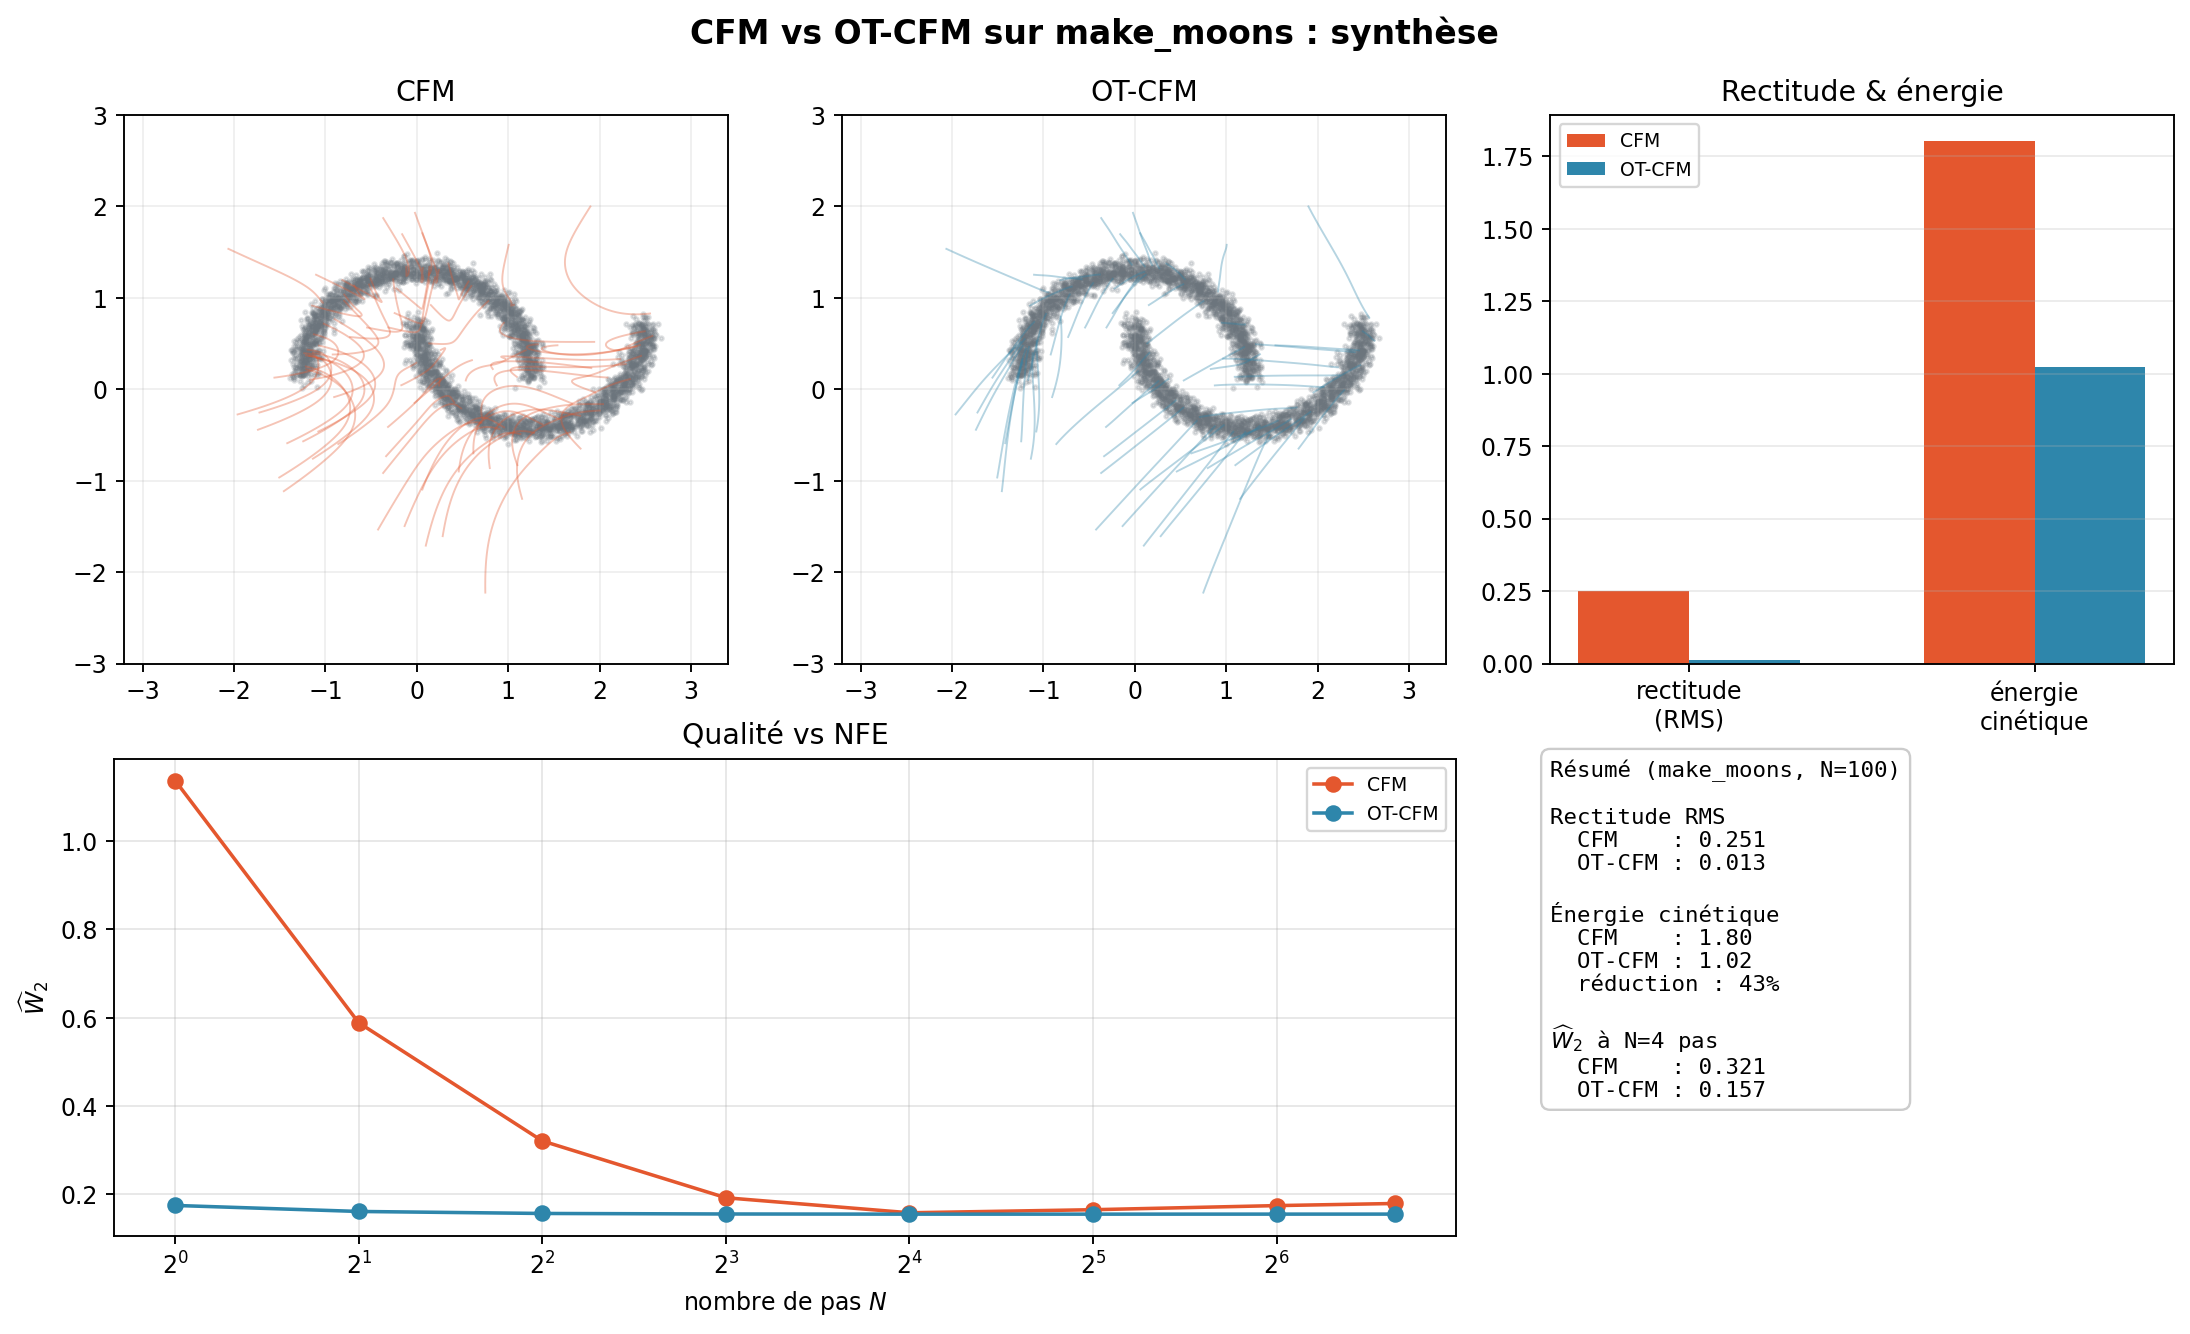
\includegraphics[width=0.95\linewidth]{figures/cfm_vs_otcfm_summary.png}
  \caption{Synthèse de la comparaison sur \texttt{make\_moons} : trajectoires, rectitude, énergie
  cinétique et qualité en fonction du NFE.}
  \label{fig:cfm-otcfm-summary}
\end{figure}

\subsection{Sur MNIST : qualité visuelle à faible NFE}

On répète l'expérience avec le U-Net (\S\,12) entraîné sur MNIST, en couplant l'OT en minibatch
directement dans l'espace pixel $\R^{784}$ (\S\,\ref{sec:ot-flow-matching}, comme à la
Figure~\ref{fig:ot-mnist-vectors}).

\begin{figure}[htbp]
  \centering
  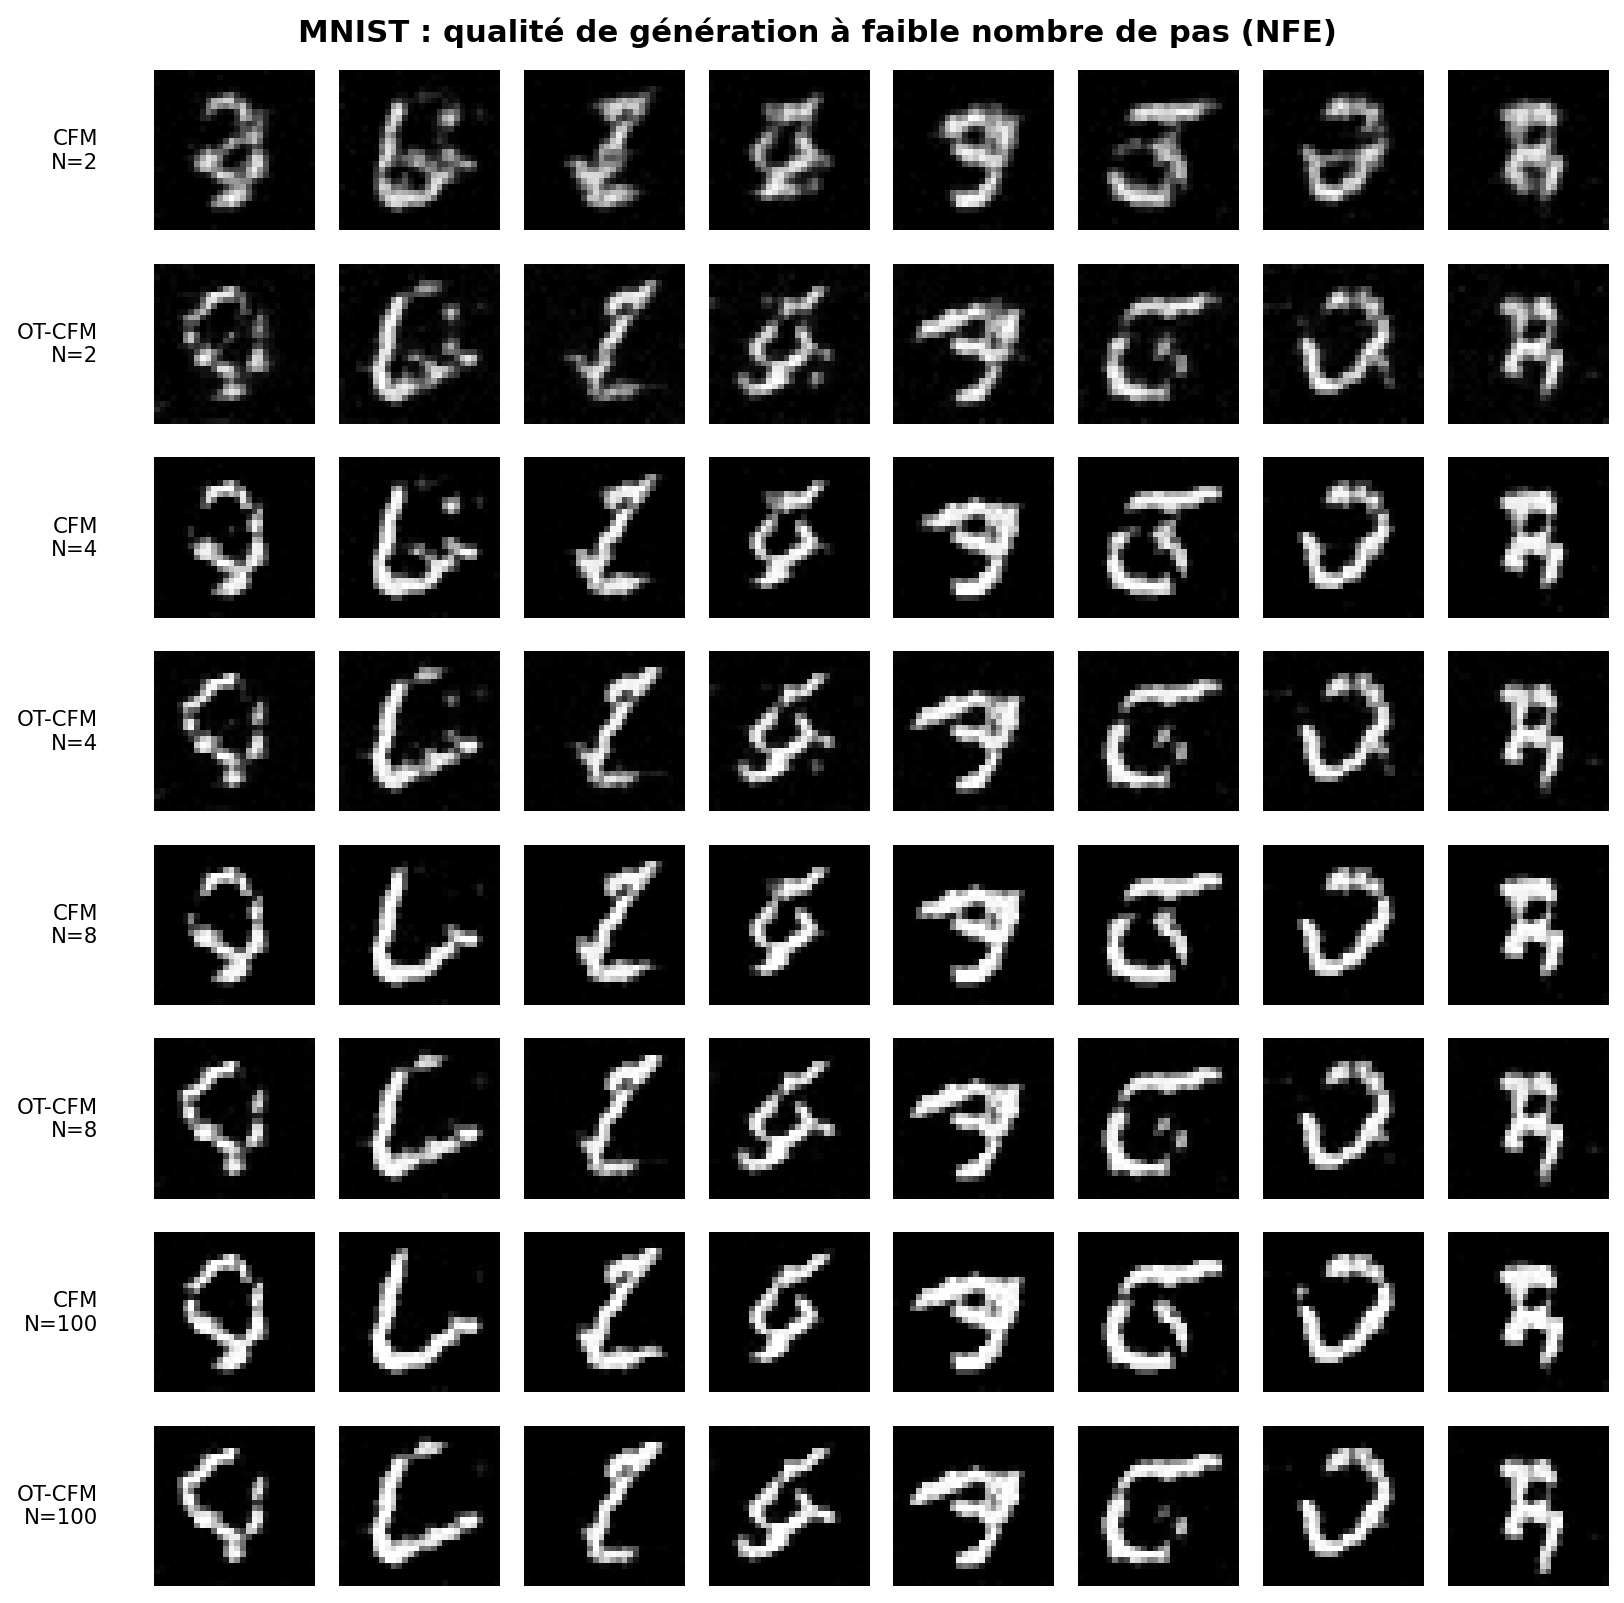
\includegraphics[width=0.92\linewidth]{figures/cfm_vs_otcfm_mnist_nfe.png}
  \caption{Échantillons MNIST générés par les modèles CFM et OT-CFM entraînés, à nombre de pas $N$
  croissant ($2$, $4$, $8$, $100$), à partir des mêmes bruits initiaux.}
  \label{fig:cfm-otcfm-mnist-nfe}
\end{figure}

\begin{warningbox}
Sur MNIST, l'écart de qualité entre CFM et OT-CFM à faible NFE est nettement moins marqué que sur
\texttt{make\_moons} : dès $N=2$ pas, les deux modèles produisent des chiffres reconnaissables de
qualité comparable. Deux raisons principales : d'une part, l'espace $\R^{784}$ est haute dimension
et le couplage OT en minibatch (taille $128$) n'y approche que très grossièrement le couplage
optimal continu du Théorème~\ref{thm:brenier} (Proposition~\ref{prop:otcfm-convergence} requiert
$m\to\infty$) ; d'autre part, la distance quadratique en espace pixel n'est pas nécessairement
celle qui gouverne la difficulté perceptuelle de la génération. Le gain de rectitude de l'OT-CFM
est donc plus net et plus facilement mesurable en basse dimension (\texttt{make\_moons}) que sur des
images brutes en pixels.
\end{warningbox}

\section{Résumé conceptuel}

\begin{enumerate}[leftmargin=*]
  \item Un flot $\Phi_t$ transporte $p_0$ vers $p_1$ au sens de l'équation de
  continuité (EC) ; c'est l'objet mathématique commun à toutes les méthodes de
  ce cours.
  \item La méthode \emph{classique} (CNF, Chen \emph{et al.}, 2018) entraîne ce
  flot par maximum de vraisemblance exacte, via la formule de changement de
  variables instantanée (Proposition~\ref{prop:instant-cov}) ; elle est
  \emph{simulation-based} : coûteuse (ODE avant et arrière, trace de jacobien,
  méthode adjointe) et sans lien direct avec l'optimalité du transport.
  \item Le flow matching choisit un couplage $\pi\in\Pi(p_0,p_{\mathrm{data}})$
  et un chemin de probabilité conditionnel affine
  $X_t=\alpha(t)X_0+\beta(t)X_1$, de vitesse exacte
  $U_t=\dot\alpha(t)X_0+\dot\beta(t)X_1$, calculable en forme close.
  \item Le champ marginal $v_t^\pi(x)=\E[U_t\mid X_t=x]$ transporte
  exactement $p_t$ (Théorème~\ref{thm:marginalisation}, par désintégration de
  $\pi$), et c'est aussi l'unique minimiseur $L^2$ de la perte de régression
  $\mathcal{L}_{\mathrm{CFM}}$ (Théorème~\ref{thm:regression}) : entraîner
  $v_\theta$ par MSE sur des cibles conditionnelles suffit donc, sans jamais
  intégrer d'ODE pendant l'entraînement -- c'est le gain \emph{simulation-free}
  par rapport au CNF.
  \item Le couplage indépendant $\pi=p_0\otimes p_1$, utilisé par défaut,
  n'atteint pas l'énergie cinétique minimale du Théorème~\ref{thm:BB} :
  les couplages OT en minibatch (OT-CFM, Tong \emph{et al.}, 2023) s'en
  rapprochent, et la paramétrisation convexe (Optimal Flow Matching, Kornilov
  \emph{et al.}, 2024) l'atteint exactement grâce au théorème de Brenier
  (Théorème~\ref{thm:brenier}), au prix d'une classe de champs plus restreinte.
  \item Pour générer, on part d'un bruit $\widehat X_0\sim p_0$ et l'on intègre
  numériquement l'ODE apprise (Euler, Heun, RK4), avec une erreur globale
  contrôlée par l'ordre du schéma et le pas $\Delta t$ -- sauf pour l'OFM, où un
  unique pas suffit exactement.
  \item Expérimentalement (Section~\ref{sec:comparaison-experimentale}), le couplage OT en
  minibatch réduit bien l'énergie cinétique et rend les trajectoires quasi rectilignes sur
  \texttt{make\_moons}, ce qui permet de générer en très peu de pas ($N=1$ à $2$) une qualité que le
  couplage indépendant n'atteint qu'à $N\gtrsim 16$ pas ; l'effet est en revanche beaucoup plus
  ténu sur MNIST, où l'OT en minibatch, à taille de batch finie, n'approche que grossièrement le
  couplage optimal continu en haute dimension.
\end{enumerate}

\section{Exercices}

\subsection*{Exercice 1 --- Conditions aux bords et régularité}

Vérifier que le schedule $\alpha(t)=\cos(\tfrac{\pi}{2}t)$,
$\beta(t)=\sin(\tfrac{\pi}{2}t)$ satisfait $X_{t=0}=X_0$, $X_{t=1}=X_1$, et
montrer que $(\alpha,\beta)$ est de classe $\mathcal{C}^\infty$ sur $[0,1]$.

\subsection*{Exercice 2 --- Vitesse linéaire}

Pour $X_t=(1-t)X_0+tX_1$, montrer que $U_t=\frac{\dd X_t}{\dd t}$ ne dépend pas
de $t$, et calculer l'énergie cinétique moyenne
$\int_0^1 \E[\|U_t\|_2^2]\dd t$ en fonction de $\E[\|X_1-X_0\|_2^2]$.

\subsection*{Exercice 3 --- Variance du chemin}

Supposons $X_0,X_1$ indépendantes, centrées, de covariance $I_d$. Calculer
$\Cov(X_t)$ pour le schedule linéaire, puis pour le schedule cosinus. En déduire
pour quelle valeur de $t$ l'écart entre les deux schedules est maximal.

\subsection*{Exercice 4 --- Démonstration du théorème de marginalisation en dimension 1}

Traiter explicitement le cas $d=1$, $\pi=p_0\otimes p_1$ (couplage indépendant),
$X_t=(1-t)X_0+tX_1$. Écrire $p_t$ comme un produit de convolution de lois
renormalisées, puis retrouver $v_t^\pi(x)=\E[X_1-X_0\mid X_t=x]$ par un calcul
direct sur les densités, sans invoquer la désintégration abstraite.

\subsection*{Exercice 5 --- Ordre du schéma d'Euler}

En utilisant un développement de Taylor de la solution exacte $X_{t_{k+1}}$
autour de $t_k$, montrer que l'erreur locale du schéma d'Euler explicite est en
$O(\Delta t^2)$, puis que l'erreur globale après $N=1/\Delta t$ pas est en
$O(\Delta t)$.

\subsection*{Exercice 6 --- Mise en pratique}

Implémenter le schéma d'Euler et le schéma de Heun de la Section~\ref{sec:integration-numerique}, comparer
visuellement (nombre de pas $N=20$, $100$, $500$) la qualité des échantillons
générés sur \texttt{make\_moons}, et estimer empiriquement l'ordre de
convergence en mesurant une distance de Wasserstein empirique entre
$\widehat X_1$ et $p_{\mathrm{moons}}$ en fonction de $N$.

\subsection*{Exercice 7 --- Changement de variables instantané}

En dimension $d=1$, pour $v_t(x)=a(t)x$ (champ linéaire), résoudre
explicitement (ODE), en déduire $\Phi_t(x_0)$, puis vérifier directement, par un
calcul de densité gaussienne, la formule de la Proposition~\ref{prop:instant-cov}
lorsque $p_0=\mathcal{N}(0,1)$.

\subsection*{Exercice 8 --- Couplage optimal en dimension 1}

En dimension $d=1$, montrer que le couplage optimal du Théorème~\ref{thm:brenier}
pour le coût quadratique est donné par $T^\star=F_1^{-1}\circ F_0$, où $F_0,F_1$
sont les fonctions de répartition de $p_0,p_1$ (couplage monotone). Comparer,
sur un petit exemple numérique à deux composantes gaussiennes pour $p_1$, la
trajectoire donnée par ce couplage à celle du couplage indépendant, et calculer
l'écart d'énergie cinétique prédit par le Théorème~\ref{thm:BB}.

\section{Ouverture}

Le flow matching présenté ici repose sur des chemins conditionnels affines
entre bruit et données, affinés par des couplages de transport optimal
(Section~\ref{sec:ot-flow-matching}). Plusieurs extensions actives en recherche
méritent encore d'être mentionnées :

\begin{itemize}[leftmargin=*]
  \item \textbf{Rectified flow} (Liu \emph{et al.}, 2022) : on \og redresse \fg{}
  itérativement les trajectoires en ré-entraînant le modèle sur des paires
  $(\widehat X_0,\widehat X_1)$ générées par le modèle précédent, ce qui
  rapproche le couplage effectif du couplage optimal de Monge
  (Théorème~\ref{thm:BB}) sans toutefois garantir l'exactitude en un nombre fini
  d'itérations, contrairement à l'Optimal Flow Matching (\S~\ref{ssec:ofm}).
  \item \textbf{Interpolants stochastiques} (Albergo--Vanden-Eijnden, 2023) :
  cadre unifiant flow matching déterministe et diffusion stochastique, en
  ajoutant un terme brownien contrôlé au chemin conditionnel tout en conservant
  les mêmes marginales.
  \item \textbf{Guidance sans classifieur} (\emph{classifier-free guidance}) :
  extrapolation entre un champ conditionnel $v_\theta(t,x\mid c)$ et un champ non
  conditionnel $v_\theta(t,x)$ pour renforcer l'adéquation à une condition $c$
  (classe, texte, etc.) au moment de l'échantillonnage.
\end{itemize}

Mais le cœur de la méthode reste celui établi dans ce cours : après avoir vu
pourquoi la méthode classique des CNF, coûteuse en simulation, a cédé la place
au flow matching (Section~\ref{sec:cnf}), puis comment ce dernier peut lui-même
être rapproché de l'optimum du transport optimal (Section~\ref{sec:ot-flow-matching}),
retenons l'idée directrice : apprendre, par simple régression $L^2$ sur des
vitesses conditionnelles explicites, un champ de vitesse marginal qui transporte
rigoureusement une distribution simple vers la distribution des données.

\section*{Références}
\begin{itemize}[leftmargin=*]
  \item R. T. Q. Chen, Y. Rubanova, J. Bettencourt, D. Duvenaud (2018),
  \emph{Neural Ordinary Differential Equations}, NeurIPS. (Continuous
  Normalizing Flows, méthode adjointe.)
  \item W. Grathwohl, R. T. Q. Chen, J. Bettencourt, I. Sutskever, D. Duvenaud
  (2018), \emph{FFJORD: Free-form Continuous Dynamics for Scalable Reversible
  Generative Models}, arXiv:1810.01367.
  \item J.-D. Benamou, Y. Brenier (2000), \emph{A computational fluid mechanics
  solution to the Monge-Kantorovich mass transfer problem}, Numerische
  Mathematik.
  \item Y. Brenier (1991), \emph{Polar factorization and monotone rearrangement
  of vector-valued functions}, Communications on Pure and Applied Mathematics.
  \item Y. Lipman, R. T. Q. Chen, H. Ben-Hamu, M. Nickel, M. Le (2023),
  \emph{Flow Matching for Generative Modeling}, arXiv:2210.02747.
  \item A. Tong, N. Malkin, G. Huguet, Y. Zhang, K. Fatras, J. Rector-Brooks,
  G. Wolf, Y. Bengio (2023), \emph{Improving and generalizing flow-based
  generative models with minibatch optimal transport}, arXiv:2302.00482.
  \item N. Kornilov, P. Mokrov, A. Gasnikov, A. Korotin (2024), \emph{Optimal
  Flow Matching: Learning Straight Trajectories in Just One Step},
  arXiv:2403.13117.
  \item X. Liu, C. Gong, Q. Liu (2022), \emph{Flow Straight and Fast: Learning
  to Generate and Transfer Data with Rectified Flow}, arXiv:2209.03003.
  \item M. S. Albergo, E. Vanden-Eijnden (2023), \emph{Building Normalizing
  Flows with Stochastic Interpolants}, arXiv:2209.15571.
  \item B. Amos, L. Xu, J. Z. Kolter (2017), \emph{Input Convex Neural
  Networks}, arXiv:1609.07152.
  \item C. Villani (2003), \emph{Topics in Optimal Transportation}, American
  Mathematical Society.
\end{itemize}

\end{document}
